%-------------------------------------------------------------------------------
% Prior abstract
%-------------------------------------------------------------------------------

We present the problem of class hierarchy complementation: given a
partially known hierarchy of classes together with subtyping
constraints (``A has to be a transitive subtype of B'') complete the
hierarchy so that it satisfies all constraints. The problem has immediate
practical application to the analysis of partial programs---e.g., it
arises in the process of providing a sound handling of ``phantom
classes'' in the Soot program analysis framework. We provide
algorithms to solve the hierarchy complementation problem in the
single inheritance and multiple inheritance settings.
% We show that class
% hierarchy complementation is NP-complete for multiple
%inheritance/subtyping while there is a polynomial algorithm for single
% subtyping hierarchies.
We also show that the problem in a language such as Java, with single
inheritance but multiple subtyping and distinguished class
vs. interface types, can be decomposed into separate single- and
multiple-subtyping instances.  We implement our algorithms in a
tool, JPhantom, which complements partial Java bytecode programs so that
the result is guaranteed to satisfy the Java verifier
requirements. JPhantom is highly scalable and runs in mere seconds
even for large input applications and complex constraints (with a maximum
of 14s for a 19MB binary).


%Static whole-program analysis requires the availability of every class
%transitively referenced in a program, even if it is never used. For
%instance, trying to analyze a program P that uses a small part of a
%third-party library L also requires the full code of any library L'
%that different parts of L may reference---the fact that L' is not
%necessary for P cannot be determined before the analysis of P is
%performed. This is a oft-encountered practical challenge, motivating
%mechanisms such as the ``phantom class'' facility in the well-known
%Soot analysis framework for Java.
%
%To address this challenge in full generality we define the problem of
%``program complementation'': given a partial program we seek to
%provide definitions for its missing parts so that the ``complement''
%satisfies all static and dynamic typing requirements induced by the
%code under analysis. This requires satisfying constraints relative to
%methods and fields of the missing classes, as well as subtyping
%constraints and constraints on whether a missing type has to be a
%class or interface. We formulate the problem systematically and offer
%an algorithm that produces solutions for the resulting constraints.
%The result is the articulation of a novel typing problem in the OO
%context, as well as a tool of practical interest. We show that we
%produce practical complements of significant size in a few seconds
%and, in this way, allow the analysis of previously un-analyzable
%partial programs.


%-------------------------------------------------------------------------------
% Introduction
%-------------------------------------------------------------------------------

\section{Introduction}
\label{intro}

Whole-program static analysis is essential for clients that require
high-precision
%in analysis results
and a deeper understanding of program behavior. Modern applications of
program analysis, such as large scale refactoring tools
\cite{journals/software/Dig11}, race and deadlock detectors
\cite{pldi/NaikAW06}, and security vulnerability detectors
\cite{sigsoft/MadsenLF13,uss/GuarnieriL09}, are virtually
inconceivable without whole-program analysis.

For whole-program analysis to become truly practical, however, it
needs to overcome several real-world challenges. One of the somewhat
surprising real-world observations is that whole-program analysis
requires the availability of much more than the ``whole program''.
The analysis needs an overapproximation of what constitutes the
program. Furthermore, this overapproximation is not merely
what the analysis computes to be the ``whole program'' after it
has completed executing. Instead, the overapproximation needs to be
as conservative as required by any intermediate step of the analysis,
which has not yet been able to tell, for instance, that some method
is never called.

Consider the example of trying to analyze a program $P$ that uses a
third-party library $L$. Program $P$ will likely only need small parts
of $L$.  However, other, entirely separate, parts of $L$ may make use
of a second library, $L'$.  It is typically not possible to analyze
$P$ with a whole program analysis framework without also supplying the
code not just for $L$ but also for $L'$, which is an unreasonable
burden. In modern languages and runtime systems, $L'$ is usually not
necessary in order to either compile $P$ or run it under any
input. The problem is exacerbated in the current era of large-scale
library reuse.  In fact, it is often the case that the user is not
even aware of the existence of $L'$ until trying to analyze $P$.

Unsurprisingly, the issue has arisen before, in different guises.  The
FAQ document\footnote{http://www.sable.mcgill.ca/soot/faq.html} of the
well-known Soot framework for Java
analysis \cite{vall99soot,valleerai00optimizing} contains the
question:

\vspace{-1mm}
\begin{quote}
\emph{How do I modify the code in
order to enable soot to continue loading a class even if it doesn't
find some of it[s] references? Can I create a dummy soot class so it can
continue with the load? How?}
\end{quote}

\noindent This frequently asked question does not lead to a solution. The answer
provided is:
\begin{quote}
\emph{You can try -use-phantom-refs but often that
does not work because not all analyses can cope with such
references. The best way to cope with the problem is to find the
missing code and provide it to Soot.}
\end{quote}

The ``phantom refs'' facility of Soot, referenced in the above answer,
attempts to model missing classes (\emph{phantom classes}) by
providing dummy implementations of their methods referenced in the
program under analysis. However, there is no guarantee that the
modeling is in any way sound, i.e., that it satisfies the well-formedness
requirements that the rest of the program imposes on the phantom
class.

Our research consists precisely of addressing the above need in full
generality. \emph{Given a set of Java class and interface definitions,
in bytecode form, we compute a ``program complement'', i.e., skeletal
versions of any referenced missing classes and interfaces so that the
combined result constitutes verifiable Java bytecode.} Our solution to
this practical problem has two parts:

\begin{asparaitem}[$\cdot$]
\item A \emph{program analysis} part, requiring analysis of bytecode and techniques
similar to those employed by the Java verifier and Java
decompilers. This analysis computes constraints involving the missing
types. For instance, if a variable of a certain type $C$ is
direct-assigned to a variable of a type $S$, then $C$ must be a subtype of
$S$.
%, as well as constraints on members (e.g., we may know from
%available bytecode that a missing class has a method with a given
%signature)

\item An \emph{algorithmic} part, solving a novel typing problem, which we call
  the \emph{class hierarchy complementation}, or
  simply \emph{hierarchy complementation}, problem. The problem
  consists of computing a type hierarchy that satisfies a set of
  subtyping constraints \emph{without} changing the direct parents of
  known types.
\end{asparaitem}


%We model all requirements on missing classes or interfaces
%(which we call ``phantom types'', alluding to the Soot terminology) as
%a set of typing constraints.

The algorithmic part of our solution, i.e., solving the hierarchy
complementation problem, constitutes the main novelty of our
approach. The problem appears to be fundamental, and even of a certain
interest in purely graph-theoretic terms. For a representative special
case, consider an object-oriented language with multiple inheritance
(or, equivalently, an interface-only hierarchy in Java or
C\#).\footnote{We avoid the terms ``subclassing'' or ``inheritance''
as synonyms for ``direct subtyping'' to prevent confusion with other
connotations of these terms. In our context, we only care about the
concept of subtyping, i.e., of a (monomorphic) type as a special case
of another. Subtyping can be direct (e.g., when a Java class is
declared to ``extend'' another or ``implement'' an interface) or
indirect, i.e., transitive. We do, however, use the compound terms
``single inheritance'' and ``multiple inheritance'' as they are more
common in the classification of languages than ``single subtyping''
and ``multiple subtyping''.}  A partial hierarchy, augmented with
constraints, can be represented as a graph, as shown in
Figure~\ref{fig:ex0:problem}. The known part of the hierarchy is shown
as double circles and solid edges. Unknown (i.e., missing) classes are
shown as single circles. Dashed edges represent subtyping constraints,
i.e., indirect subtyping relations that have to hold in the resulting
hierarchy. In graph-theoretic terms, a dashed edge means that there is
a path in the solution between the two endpoints. For instance, the
dashed edge from $C$ to $D$ in Figure~\ref{fig:ex0:problem} means that
the unknown part of the class hierarchy has a path from $C$ to
$D$. This path cannot be a direct edge from $C$ to $D$, however: $C$
is a known class, so the set of its supertypes is fixed.

\begin{figure}[t]
  \begin{minipage}[b]{.5\linewidth}
    \centering
    \includegraphics[scale=0.6]{figures/complementation/cgraph2.pdf}
    \subcaption{Constraint Graph}\label{fig:ex0:problem}
  \end{minipage}
  \begin{minipage}[b]{.5\linewidth}
    \centering
    \includegraphics[scale=0.6]{figures/complementation/cgraph2-solution.pdf}
    \subcaption{Solution}\label{fig:ex0:solution}
  \end{minipage}
  \caption[Example of constraints in a multiple inheritance setting]{%
    Example of constraints in a multiple inheritance
    setting. Double-circles signify known classes, single circles
    signify unknown classes. Solid edges (``known edges'') signify
    direct subtyping, dashed edges signify transitive subtyping.}
  \label{fig:ex0}
\end{figure}

In order to solve the above problem instance, we need to compute a
directed acyclic graph (DAG) over the same nodes,\footnote{Inventing
extra nodes does not contribute to a solution in this problem.} so
that it preserves all known nodes and edges, and adds edges \emph{only
to unknown nodes} so that all dashed-edge constraints are
satisfied. That is, the solution will not contain dashed edges
(indirect subtyping relationships), but every dashed edge in the input
will have a matching directed path in the solution
graph. Figure~\ref{fig:ex0:solution} shows one such possible solution.
As can be seen, solving the constraints (or determining that they are
unsatisfiable) is not trivial. In this example, any solution has to
include an edge from $B$ to $E$, for reasons that are not immediately
apparent. Accordingly, if we change the input of
Figure~\ref{fig:ex0:problem} to include an edge from $E$ to $B$, then
the constraints are not satisfiable---any attempted solution
introduces a cycle. The essence of the algorithmic difficulty of the
problem (compared to, say, a simple topological sort) is that we
cannot add extra direct parents to known classes $A$ and $C$---any
subtyping constraints over these types have to be satisfied via
existing parent types. This corresponds directly to our high-level
program requirement: we want to compute definitions for the missing
types only, without changing existing code.

% We show that computing whether such a DAG exists is an
% NP-complete problem, for the case of multiple subtyping.

For a language with single inheritance, the problem is similar, with
one difference: the solution needs to be a tree instead of a DAG. (Of
course, the input in Figure~\ref{fig:ex0:problem} already violates the
tree property since it contains known nodes with multiple known
parents.) We offer an algorithm that solves the problem by
either detecting unsatisfiability or always ordering the nodes in a
tree that respects all constraints.

%\footnote{Although this is true only because we are accepting any
%legal bytecode as input. As we discuss later, if we assume that the
%input is produced by following specific compiler conventions
%then...}

The practical version of the hierarchy complementation problem is more
complex. Mainstream OO languages often distinguish between classes and
interfaces and only allow single direct subtyping among classes and
multiple direct subtyping from a class/interface to an interface---a
combination often called ``single-inheritance, multiple
subtyping''. In this case, the graph representation of the problem is
less intuitive. Consider Figure~\ref{fig:real-example:problem} that
gives a problem instance. (A possible solution for these constraints
is in Figure~\ref{fig:real-example:solution}, but is given purely for
reference, as it is not central to our discussion.) There are now
several node types: classes, interfaces (both known and unknown), as
well as undetermined nodes. There are also more implicit constraints
on them: classes can only have an edge to one other class, interfaces
can only have edges to other interfaces.  The latter constraint, for
instance, forces $D$ to be an interface and $H$ to be a class. Thus, we
see that the full version of the problem requires additional
reasoning. We show that such reasoning can be performed as a
pre-processing step. The problem can be subsequently broken up into
two separate instances of the aforementioned single- and
multiple-inheritance versions of hierarchy complementation.

%merely refines locally the algorithms for solving the
%problem versions for multiple inheritance and

\begin{figure}[t]
  \begin{minipage}[b]{.5\linewidth}
    \centering
    \includegraphics[scale=0.6]{figures/complementation/cgraph3.pdf}
    \subcaption{Constraint Graph}\label{fig:real-example:problem}
  \end{minipage}
  \begin{minipage}[b]{.5\linewidth}
    \centering
    \includegraphics[scale=0.6]{figures/complementation/solution3.pdf}
    \subcaption{Solution}\label{fig:real-example:solution}
  \end{minipage}
  \caption[Example of full-Java constraint graph]{Example of full-Java
    constraint graph. Double circles denote known classes/interfaces,
    whose outgoing edges in the solution are already determined (solid
    input edges). White nodes are classes, black nodes are interfaces,
    grey nodes are unknown types that are initially undetermined
    (i.e., the input does not explicitly identify them as classes or
    interfaces, although constraint reasoning may do so later).}
  \label{fig:real-example}
\end{figure}



% Subsequently, we offer an algorithm for
% solving program complementation constraints. We implement our solution
% for Java, at the bytecode level. Our resulting tool accepts as
% input a set of Java bytecode files and produces a jar file with
% appropriate definitions of all phantom types.

%% The well-formedness guarantee of our solution to the program
%% complementation problem is that we produce classes that could have
%% been produced by the front-end Java compiler (javac) for \emph{some}
%% definition of phantom classes. This offers no guarantee that the
%% resulting original program + complement will not exhibit dynamic type
%% errors, but such a guarantee is not required: the assumption is that
%% phantom classes are indeed \emph{not used} in a meaningful way, and
%% all we want is for them to be consistent with the rest of the
%% program. For instance, a key consistency property of our solution
%% relative to the Soot phantom class treatment is that we respect
%% subtyping: if a subtyping relationship involving a phantom class
%% (or interface) can be inferred from the code then it is satisfied
%% in the complement that we output.

% To see why the problem has interesting depth and complexity, consider
% a simple fragment of Java bytecode and the constraints it
% induces. Our convention throughout the paper is that single-letter
% class names at the lower end of the alphabet (\code{A}, \code{B},
% ...)  correspond to known types, while class names at the high end
% of the alphabet (\code{X}, \code{Y}, \code{Z}) denote phantom types.
% We present bytecode in a slightly condensed form, to make clear what
% method names or type names are referenced in every instruction.
%
% \begin{smallnolinecode}
% \begin{verbatim}
% public void foo(X, Y);
%  0: aload_2     // load on stack 2nd argument (of type Y)
%  1: aload_1     // load on stack 1st argument (of type X)
%  2: invokevirtual X.bar:(LA;)LZ; //method 'Z bar(A)' in X
%  3: checkcast B // cast the result of the call to B
%  ...
% \end{verbatim}
% \end{smallnolinecode}
%
% Although the above fragment is merely four bytecode instructions
% long, it induces several interesting constraints for our phantom
% types \code{X}, \code{Y}, and \code{Z}:
%
% \begin{bullets}
% \item \code{X} has to support a method \code{bar} accepting an
%   argument of type \code{A} and returning a value of type \code{Z}.
%
% \item \code{Y} has to be a subtype of \code{A}, since an actual
%   argument of declared type \code{Y} is passed to \code{bar}, which
%   has a formal parameter of type \code{A}. This constraint also
%   means that if \code{A} is known to be a class (and not an
%   interface) then \code{Y} is also a class.
%
% \item \code{Z} is either a subtype of \code{B} or a supertype of
%   \code{B}.  The reason is that we have a cast from a reference of
%   type \code{Z} to one of type \code{B} and our well-formedness
%   requirements dictate that no dynamic type error (class cast
%   exception) be produced by such a cast. A naive view would suggest
%   that the real constraint induced by the cast is that \code{Z} be a
%   supertype of \code{B} (since the existence of a dynamic cast check
%   implies a narrowing conversion) but the bytecode may elide any
%   number of intermediate casts that existed in the source code. For
%   instance, the source code may have cast the return value of
%   \code{bar} to \code{java.lang.Object} (a cast that is always safe
%   and thus disappears in the bytecode) before casting it to
%   \code{B}. Thus, the real constraint is that \code{Z} (which is
%   only the static type of the reference, and therefore a supertype
%   of the dynamic type of the object) is either a subtype or
%   supertype of \code{B}.
% \end{bullets}
%
% Our approach will create skeletal versions of \code{X}, \code{Y},
% and \code{Z} so that all the above requirements are
% satisfied. Clearly, there can be unsatisfiable instances of the
% above constraints (e.g., cyclic subtyping requirements), and these
% are detected by our algorithm. However, unsatisfiable constraints
% cannot arise in real-world instances of the problem, unless parts of
% the code have changed without recompiling other, dependent parts.

In brief, the contributions of our work are as follows:

\begin{itemize}[--]
\item We introduce a new typing problem, motivated by real-world needs
  for whole program analysis. To our knowledge, the hierarchy
  complementation problem has not been studied before, in any context.
\item We produce algorithms that solve the problem in three different
  settings: single inheritance, multiple inheritance, and mixture of
  the two, as in Java or C\#.
%  For a single inheritance setting, we
%  offer a simple algorithm, possibly of wider applicability to other
%  domains (e.g., partially-ordered sets for which the concept of
%  ``direct predecessor'' needs to be distinguished from merely ``in
%  order''). Based on similar insights, we adapt the algorithm to a
%  multiple inheritance setting.
%  For the practical setting of a single-inheritance,
%  multiple-subtyping language, we offer an algorithm that decomposes
%  the problem into the previous two versions.
%, and also prove
% that the problem is NP-complete.
%  we offer an algorithm
%  that has exponential complexity in the worst case.
\item We implement our algorithms in JPhantom: a practical tool for
  Java program complementation that addresses the soundness
  shortcomings of previous Java ``phantom class'' approaches. We show
  that JPhantom scales well and takes only a few seconds to process
  even large benchmarks with complex constraints---e.g., less than
  6sec for a 3.2MB binary that induces more than 100 constraints.
%, encountering no exponential complexity
%  in practice.
\item We discuss the problem of hierarchy complementation in more
  general settings. The simplicity of our approach is a result of only
  assuming (for the input) and satisfying (for the output) the fairly
  weak Java bytecode requirements. We show that the problem becomes
  harder at the level of the type system for the source language.
\end{itemize}


%-------------------------------------------------------------------------------
% Motivation
%-------------------------------------------------------------------------------

% In the next sections we detail
\section{Motivation and Practical Setting}

We next discuss the practical setting that gives rise to the hierarchy
complementation problem.

Our interest in hierarchy complementation arose from efforts to
complement existing Java bytecode in a way that satisfies the
soundness guarantees of the Java verifier. Consider a small fragment
of known Java bytecode and the constraints it induces over unknown
types. (We present bytecode in a slightly condensed form, to make
clear what method names or type names are referenced in every
instruction.) In this code, classes \code{A} and \code{B} are
available, while types \code{X}, \code{Y}, and \code{Z} are phantom,
i.e., their definition is missing.

\begin{bytecode}
public void foo(X, Y)
0: aload_2     // load on stack 2nd argument (of type Y)
1: aload_1     // load on stack 1st argument (of type X)
2: invokevirtual X.bar:(LA;)LZ; // method 'Z bar(A)' in X
3: invokevirtual B.baz:()V;     // method 'void baz()' in B
 ...
\end{bytecode}

The instructions of this fragment induce several constraints for our phantom
types. For instance:

\begin{itemize}[--]
\item \code{X} has to be a class (and not an interface) since it
  contains a method called via the \code{invokevirtual} bytecode
  instruction.
\item \code{X} has to support a method \code{bar} accepting an
  argument of type \code{A} and returning a value of type \code{Z}.
\item \code{Y} has to be a subtype of \code{A}, since an actual
  argument of declared type \code{Y} is passed to \code{bar}, which
  has a formal parameter of type \code{A}. This constraint also means
  that if \code{A} is known to be a class (and not an interface) then
  \code{Y} is also a class.
\item \code{Z} has to be a subtype of \code{B}, since a method of
  \code{B} is invoked on an object of declared type \code{Z} (returned
  on top of the stack by the earlier invocation).
\end{itemize}

The goal of our JPhantom tool is to satisfy all such constraints and
generate definitions of phantom types \code{X}, \code{Y}, and \code{Z}
that are compatible with the bytecode that is available to the tool
(i.e., exists in known classes). Compatibility with existing bytecode
is defined as satisfying the requirements of the Java verifier, which
concern type well-formedness.

Of these constraints, the hardest to satisfy are those involving
subtyping.  Constraints on members (e.g., \code{X} has to contain a
``\code{Z bar(A)}'') are easy to satisfy by just adding type-correct
dummy members to the generated classes. This means that the problem in
the core of JPhantom is solving the class hierarchy complementation
problem, as presented in the introduction and defined rigorously in
later sections. The binding of the problem to practical circumstances
deserves some discussion, however.

First, note that, in our setting of the problem, we explicitly
disallow modification of known code, e.g., in order to remove
dependencies, or to add a supertype or a member to it. Such
modifications would have a cascading effect and make it hard to argue
about what properties are really preserved. Additionally, we do not
assume any restrictions on the input, other than the well-formedness
condition of being legal Java bytecode (according to the
verifier). Strictly speaking, our well-formedness condition for the
input is defined as follows: \emph{a legal input is bytecode that can
  be complemented (by only adding extra class and interface
  definitions) so that it passes the Java verifier}. Note that this
well-formedness condition does not depend on the program complement
that our approach produces: an input is legal if there is \emph{some}
complement for it, not necessarily the one that JPhantom computes.

%%% We later use this. Better not emphasize it.
%Notably, this well-formedness condition does
%not assume that known classes have known superclasses---e.g.,
%Figure~\ref{fig:real-example:problem} offered an instance where a
%superclass was a phantom type. Of course, an actual usage setting of
%JPhantom can impose this or other restrictions on the input.

% There
%are several good reasons for this decision: First, modification of
%existing code would likely
%-we cannot modify existing code. E.g., adding a supertype induces
%constraints that are not satisfied (e.g., an interface method may not be
%implemented).

A final interesting point concerns the practical impact of the
JPhantom soundness condition. For most program analyses, omitting
parts of the code introduces unsoundness, if we make no other
assumptions about the program or the omitted part. E.g., it is
impossible to always soundly compute points-to information, or
may-happen-in-parallel information when part of the program is
missing. Therefore, guaranteed soundness for all clients is inherently
unachievable for \emph{any} partial program analysis approach. The
practical reality is that there is a large need for facilities for
handling partial programs. For instance, the Soot phantom class
machinery has been one of the most common sources of discussion and
questions on the Soot support lists, and it has been a central part of
several Soot revisions.\footnote{Even the most recent Soot release,
2.5.0, lists improved support for phantom classes and excluding
methods from an analysis as one of the major changes in the release
notes.} The only ``correctness condition'' that Soot phantom class
support is trying to achieve, however, is the low-level ``the analyzer
should not crash''.

Given the practical interest for the solution of a worst-case
unsolvable problem, we believe that our soundness guarantee makes a
valuable contribution: it is much better to analyze a partial program
in a way such that the Java verifier requirements (for type-level
well-formedness) are satisfied than to ignore any correctness
considerations, as past approaches do.

% unsatisfiable constraints cannot arise in
%real-world instances of the problem, unless parts of the code have
%changed without recompiling other, dependent parts.


%-------------------------------------------------------------------------------
% Multiple Inheritance
%-------------------------------------------------------------------------------

\section{Hierarchy Complementation for Multiple Inheritance}
\label{multiple}

We begin with a modeling of the hierarchy complementation problem in
the setting of multiple inheritance. This means that every class in our
output can have multiple parents.

%% Formalization

We can model our problem as a graph problem. Our input is a directed
graph $G = (V,E)$, with two disjoint sets of nodes $V = V_{known} \disjunion
V_{phantom}$ and two disjoint sets of edges $E = E_{direct} \disjunion
E_{path}$, where $E_{direct} \subseteq V_{known} \times V$ (i.e.,
direct edges have to originate from known nodes---the converse is not
true, as known nodes can be inferred to subtype unknown ones due to
assignment instructions in the bytecode). The set of nodes $V$ is a
set of types, while the set of edges $E$ corresponds to our subtyping
constraints. That is, an edge $(v_s,v_t)$ encodes the constraint $v_s
<: v_t$. The $E_{direct}$ subset encodes the direct-subtype
constraints. The output of our algorithm should be a \emph{DAG} (with
edges from children to their parents), $G_D = (V,E')$, such that:
\begin{enumerate}
\item $\forall v_s \in V_{known}: (v_s,v_t) \in E' \Leftrightarrow (v_s,
 v_t) \in E_{direct}$ (i.e., all direct edges from known nodes are preserved
and no new ones are added to such nodes)
\item $(v_s,v_t) \in E_{path} \Rightarrow$ there is a path from $v_s$ to
$v_t$ in $G_D$
\end{enumerate}

%Again, we could decouple path-edges from direct-edges by introducing
%the input and output mappings, $f_i:V_{known} \rightarrow 2^V$,
%$f_o:V \rightarrow 2^V$. In both cases, these two mappings map a type
%(key) to its \emph{set} of outgoing edges (value). This way, $G_C =
%(V,E)$ will only contain path-edges such that $\forall (x_1,x_n) \in E
%:$ there must exist a path $(x_1,x_2,\ldots,x_n) \text{ in }
%G_D$ (second constraint). Additionally, as in the single inheritance case, we must ensure
%that $\forall c \in V_{known}: f_o[c] = f_i[c]$ (first constraint).

Note that our only limiting constraint here is that we cannot have
cycles in the resulting hierarchy. Moreover, since each type may have
multiple supertypes in this setting, a directed acyclic graph is
fitting as our intended output.

%% Phantom-only case

In contrast to the general case, the problem is trivial if we have a
phantom-only input, i.e., if we ignore $V_{known}$ and
$E_{direct}$. It suffices to employ a cycle-detection algorithm,
and---if no cycles are present---return the input constraint graph as
our solution: all path edges can become direct subtyping edges. If our
input graph contains a cycle, then our problem is unsolvable.  If
not, our solution would probably contain some redundant edges (i.e.,
edges connecting nodes that are already connected by another path)
that we could prune to minimize our output. In either case, our
solution would be valid w.r.t. our constraints.

%Optionally, we could prune some edges from our
%solution without breaking any constraints, to minimize the output of
%our algorithm for practical
%purposes. Algorithm~\ref{alg:multiple:simple} performs such an
%optimization, by first computing a transitive closure of the
%constraints and then removing redundant edges, whose target can be
%reached from another path.

%% Projection Sets

The problem becomes much more interesting when we take $V_{known}$
into account. The source of the difficulty is the combination of cycle
detection with nodes whose outgoing edge set cannot be extended.
Consider first the pattern of Figure~\ref{fig:choice}.

\begin{figure}[htp]
  \centering \includegraphics[scale = 0.6]{figures/complementation/minimum.pdf}
  \caption[Multiple Inheritance Constraint]{In any solution of these
    constraints, either $B$ or $C$ or $D$ have to be ordered below
    $E$, since no new outgoing edges can be added to $A$ and the path
    constraint to $E$ needs to be satisfied.}
\label{fig:choice}
\end{figure}

This pattern is a basic instance of interesting reasoning in the case of
multiple inheritance. We have $A \in V_{known}$ such that $(A,B),
(A,C), (A,D) \in E_{direct}$ and $(A,E) \in E_{path}$. We cannot,
however, satisfy the path ordering constraint by adding edges to the
known node $A$. Therefore the output must have one of $B,C,D$ ordered
below $E$. We refer to the set of $\{B,C,D\}$ as the \emph{projection
  set} of node $A$, which is a more generally useful concept.

\begin{defn}{\emph{Projection Set.}}
%  Let $G = (V,E) : V = V_{known} \disjunion V_{phantom}$ and $E
%  = E_{path} \disjunion E_{direct}$ be a constraint graph.
  A node $t \in V_{phantom}$ belongs to the \emph{projection set} of a
  node $s \in V_{known}$ iff $t$ is reachable from $s$ through a path
  of \emph{direct} edges.
  %% Redundant: (a path of direct edges will always contain known nodes
  %% internally)
  %% that internally contains only known nodes.
  %%
  %% We need the definition below since it is used in the algorithm.
 $$ \textit{proj}(s) \equiv \{t \in V_{phantom}: (s,t) \in {E_{direct}}^+\}$$
 with the $+$ symbol denoting transitive closure.
  %% This is wrong!
 %% $$ proj(s,t) \equiv \{(s,t): t \in V_{phantom} \land (s,t) \in
 %% {E_{direct}}\}^+$$ with the $+$ symbol denoting transitive
 %% closure.
\end{defn}

That is, for each known node we can follow its outgoing direct-edges
recursively, ending each path when we reach a phantom node. For
instance, in Figure~\ref{fig:proj}, the phantom projection set for
node $A$ is $\{C,E,H\}$.

% Node $I$ is not included since no path exists
% from $A$ to $I$ through direct-edges only.

Referring again to Figure~\ref{fig:proj}, we can see that if $H$ is
chosen from the projection set of $A$ in order to satisfy the
path-edge $(A,B)$, and therefore edge $(H,B)$ is added, then this
would immediately create a cycle because of the existing $(B,H)$
edge. Our algorithm should prevent such a cycle by making the correct
choice from the relevant projection set.
% Furthermore, we can also see why it is redundant to add $I$ in the
% projection set of $A$. Had node $C$ created a cycle if chosen to
% satisfy the path to node $B$ (or any other node), it would mean that
% a path from $B$ to $C$ exists, and so it would be impossible to
% satisfy the same constraint through $I$ (since there is also a path
% from $B$ to $I$, through node $C$).

\begin{figure}[tp]
  \centering
  %%\subfloat[Constraint Graph]{
    \includegraphics[scale=0.6]{figures/complementation/projections.pdf}
    %%\label{fig:proj:graph}
  %%}
  %% \subfloat[Solution]{
  %%   \includegraphics[scale=0.4]{images/stree1-ext.pdf}
  %%   \label{fig:cgraph1:ext}
  %% }
  \caption[Phantom Projection Set]{%
    The phantom projection set of $A$ is $\{C,E,H\}$. In order to
    satisfy path-edge $(A,B)$ we can either add a path-edge $(C,B)$,
    $(E,B)$, or $(H,B)$. The last one creates a cycle.
  }
\label{fig:proj}
\end{figure}

%% Multiple Inheritance Examples

Combining this projection set choice with cycle detection leads to
interesting search outcomes. Figure~\ref{fig:unsat} shows an example
of unsatisfiable input. The path edge $(B,D)$ makes either $E$ or $F$
be subtypes of $D$, and similarly the path edge $(A,C)$ makes either
$E$ or $F$ be subtypes of $C$. Nevertheless, any choice leads to
cycles. In contrast, Figure~\ref{fig:multipleHard} shows an input for
which a solution is possible, and which we use to illustrate our
algorithm.

\begin{figure}[htp]
  \begin{minipage}[b]{.5\linewidth}
    \centering
    \includegraphics[scale=0.6]{figures/complementation/multipleUnsat.pdf}
    \subcaption{Unsatisfiable input}\label{fig:unsat}
  \end{minipage}
  \begin{minipage}[b]{.5\linewidth}
    \centering
    \includegraphics[scale=0.6]{figures/complementation/multipleEx.pdf}
    \subcaption{Satisfiable input}\label{fig:multipleHard}
  \end{minipage}
  \caption{Multiple Inheritance Examples}
\end{figure}

%%% WRONG!!!
%%%%
% In the same vein, the example of Figure~\ref{fig:multipleHard} is
% satisfiable, but requires some reasoning to find a solution. The path
% edge $(B,H)$ cannot be satisfied by ordering $E$ below $H$ without
% introducing a cycle, but can be satisfied by ordering $F$ below $H$.
%%%%%

%% Algorithm explanation

Algorithm~\ref{alg:multiple:strat} solves in polynomial time (an easy bound is
$O(|V| \cdot |E|)$) any
instance of the hierarchy complementation problem in the multiple
inheritance setting. The main part of the algorithm is
function \textsc{stratify()}, which computes a stratification with the
property that any constraint edge is facing upwards (i.e., from a
lower to a higher stratum). Moreover, this stratification ensures
that, for any path-edge $(s,t)$ originating from a known node, there
will exist a phantom node $p$ in the projection set of $s$ that is
placed lower than $t$. Given this stratification, it is easy to
compute the final solution (as in function~\textsc{solve()}). To
satisfy any such path-edge $(s,t)$, we add a direct-edge from $p$ to
$t$. This respects our invariant of all edges facing upwards, thus
ensuring that no cycles will be present in our solution.

Function~\textsc{stratify()} starts from a single stratum, and then
computes on each iteration a new stratification, $S_{i+1}$, by
building on the stratification of the previous step, $S_{i}$, and
advancing some nodes to a higher stratum in order to satisfy
constraints. This process is repeated until we converge to the final
stratification, which will respect all of our constraints
(line~\ref{lst:line:fixpoint}). If no new node converges at some step
(i.e., all nodes that reached a certain stratum advance to the next),
then we can be certain that we are dealing with unsatisfiable input,
and terminate, thus avoiding infinite recursion
(line~\ref{lst:line:unsat}). The nodes to be advanced at each step are
determined at line~\ref{lst:line:formula}, which captures the essence
of the algorithm. The new stratum of a node $t$ will be either%
\begin{inparaenum}[(i)]
\item its current stratum,
\item the stratum right above the source of an edge $(s,t)$, or
\item the one right above the \emph{lowest} projection node of the
  source of a path-edge $(s,t)$ originating from a known node%
\end{inparaenum}%
---whichever is higher.  These conditions raise the stratum of a node
to the minimum required to satisfy the natural constraints of the
problem, per our above discussion: edges in the solution should be
from lower to higher strata.

%% Stratification Example

\begin{figure*}[t]
  \vspace{-5mm}
  \begin{minipage}[b]{0.5\linewidth}
    \centering
    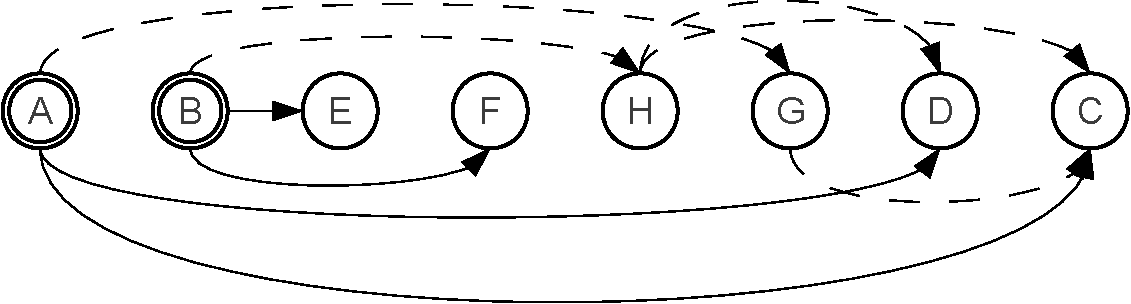
\includegraphics[scale=0.4]{figures/complementation/steps-0-crop.pdf}
    \subcaption{Step 1}\label{fig:multiple:steps:0}
  \end{minipage}
  \begin{minipage}[b]{0.5\linewidth}
    \centering
    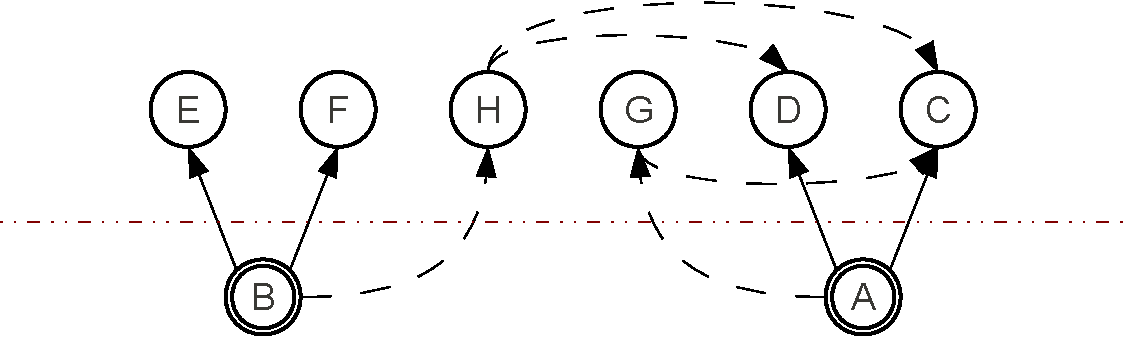
\includegraphics[scale=0.4]{figures/complementation/steps-1-crop.pdf}
    \subcaption{Step 2}\label{fig:multiple:steps:1}
  \end{minipage}
  \\
  \begin{minipage}[b]{0.5\linewidth}
    \centering
    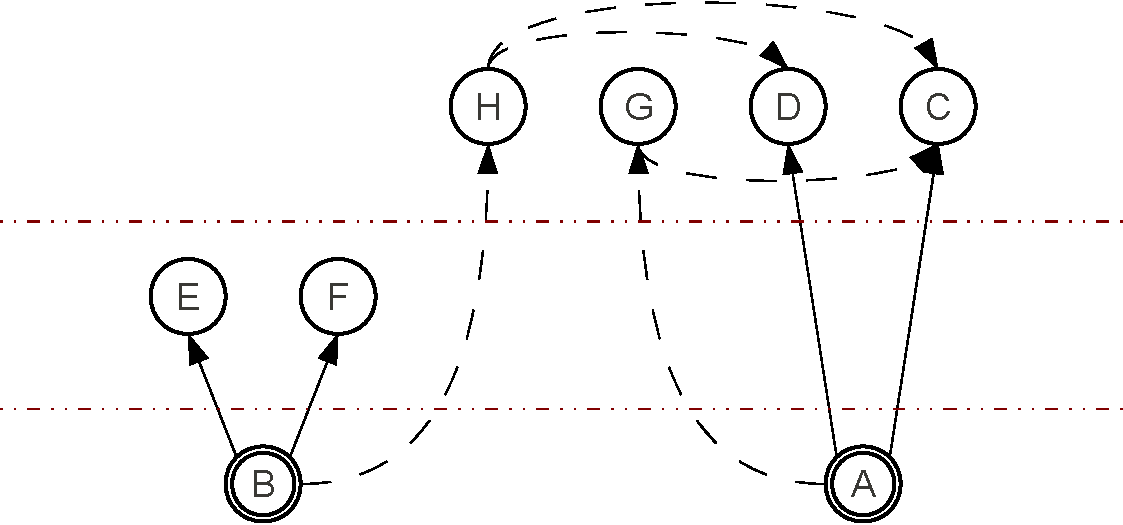
\includegraphics[scale=0.4]{figures/complementation/steps-2-crop.pdf}
    \subcaption{Step 3}\label{fig:multiple:steps:2}
  \end{minipage}
  \begin{minipage}[b]{0.5\linewidth}
    \centering
    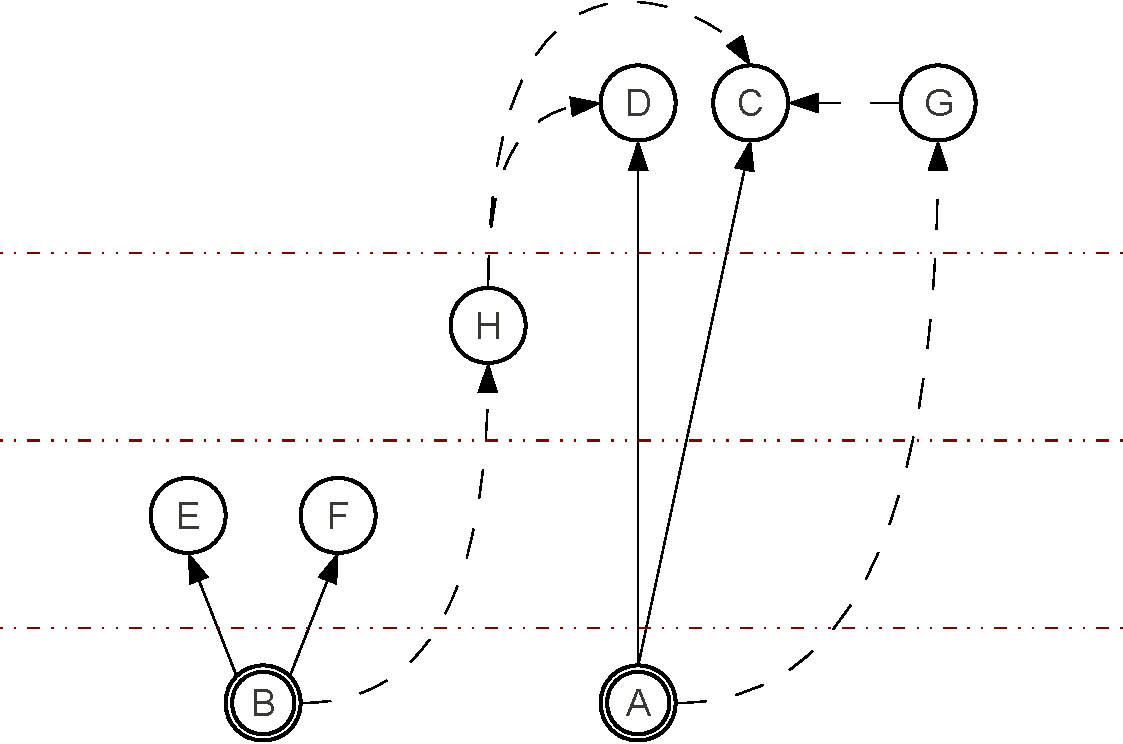
\includegraphics[scale=0.4]{figures/complementation/steps-3-crop.pdf}
    \subcaption{Step 4}\label{fig:multiple:steps:3}
  \end{minipage}
  \\
  \begin{minipage}[b]{0.5\linewidth}
    \centering
    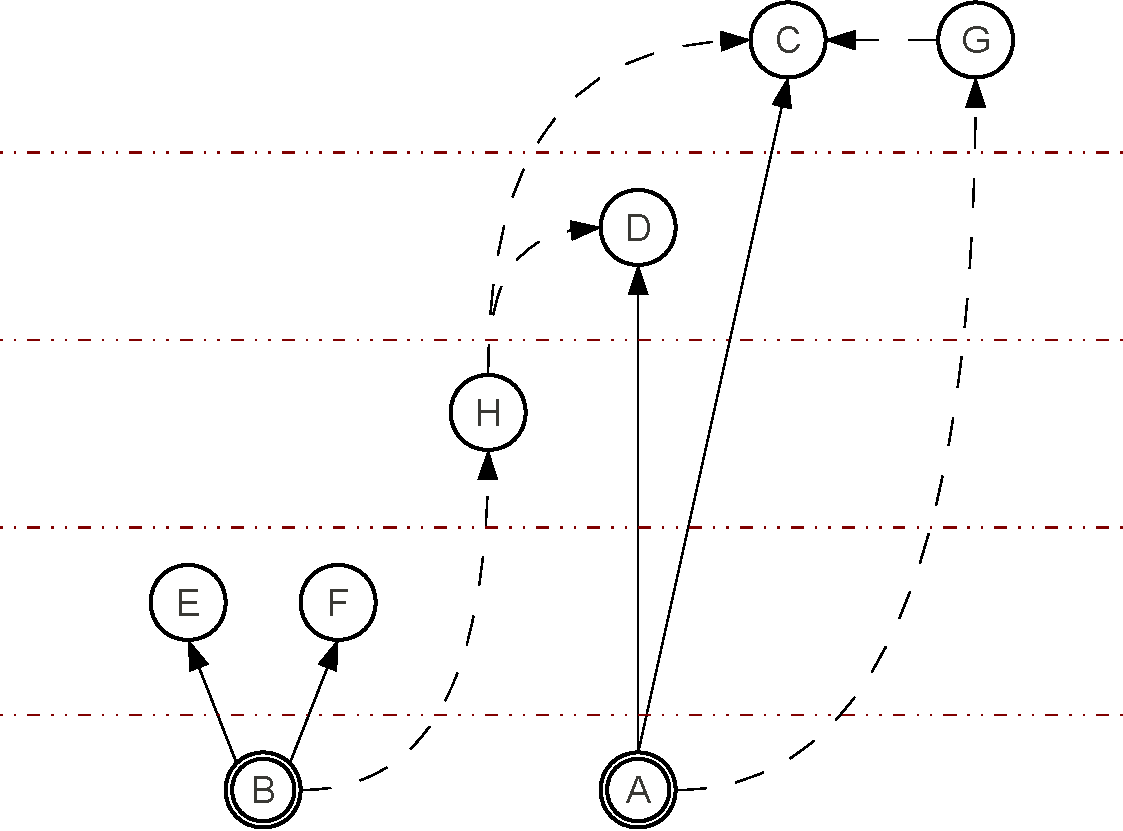
\includegraphics[scale=0.4]{figures/complementation/steps-4-crop.pdf}
    \subcaption{Step 5}\label{fig:multiple:steps:4}
  \end{minipage}
  \begin{minipage}[b]{0.5\linewidth}
    \centering
    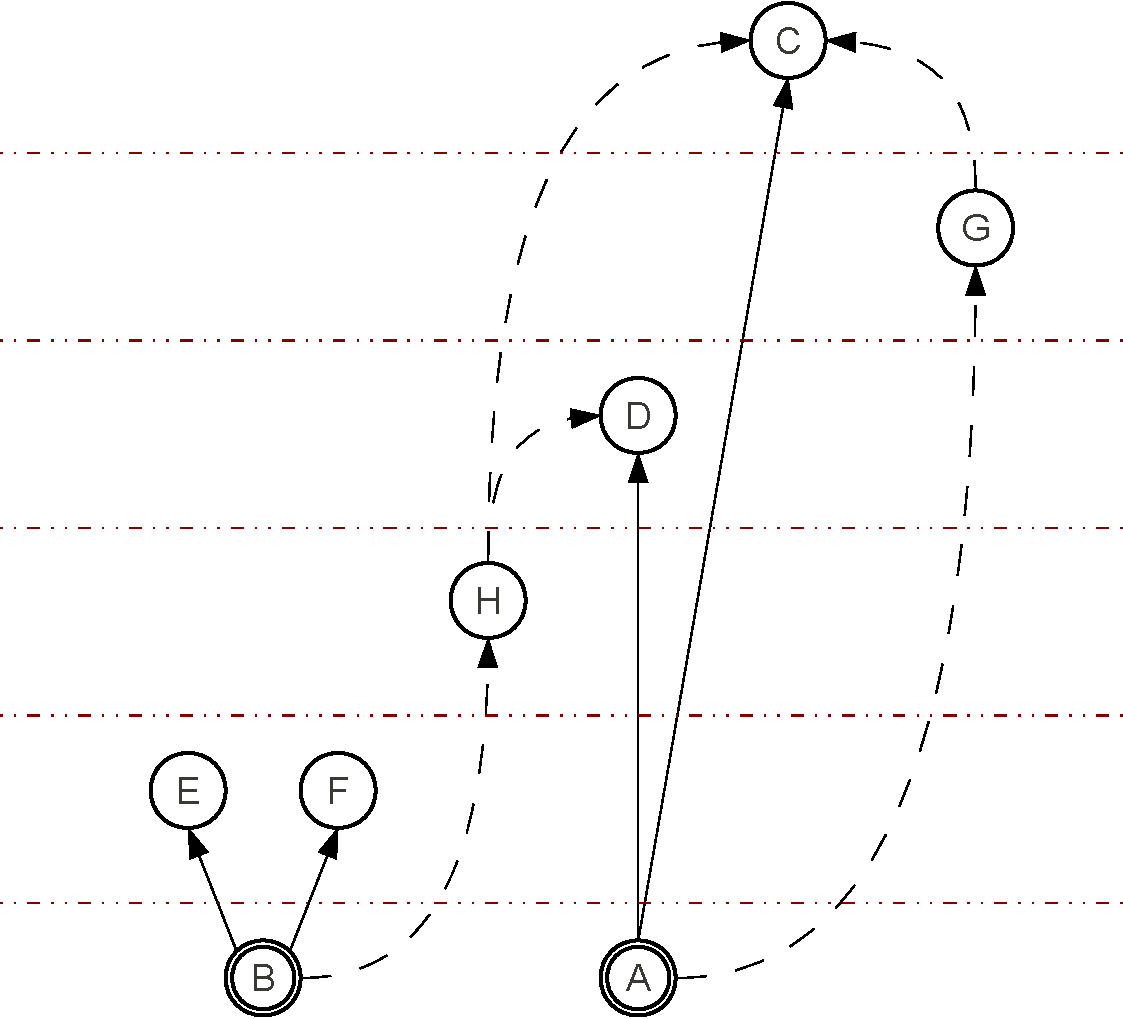
\includegraphics[scale=0.4]{figures/complementation/steps-5-crop.pdf}
    \subcaption{Step 6}\label{fig:multiple:steps:5}
  \end{minipage}
  \caption[Stratification Example]{An example of the stratification
    produced by the multiple-inheritance solver for
    Example~\ref{fig:multipleHard}.}
  \label{fig:multiple:steps}
\end{figure*}

\begin{algorithm}
  \caption{Multiple-inheritance solver}
  \label{alg:multiple:strat}
  \small

  \hrulefill

  \begin{algorithmic}[1]
    \Function{solve}{$G = (V,E)$} \Let{$S$}{\Call{stratify}{$G$}}
    \Let{$U$}{$\{(s,t) \in E_{path} : s \in V_{known}\}$}
    \Let{$E_S$}{$E \setminus U$}
    \ForAll{$(s,t) \in U$}
       \State let $p \in \textit{proj}(s) : S[p] < S[t]$
       \Comment{such $p$ always exists}
       \Let{$E_S$}{$E_S \cup \{(p,t)\}$}
    \EndFor
    \State \Return $E_S$
    \EndFunction
    \algstore{alg:strat}
  \end{algorithmic}
%  \hrulefill
  \begin{algorithmic}[1]
    \algrestore{alg:strat}
    \Function{stratify}{$G = (V,E)$}
    \Let{$U$}{$\{(s,t) \in E_{path} : s \in V_{known}\}$}
    \ForAll{$t \in V$} \Let{$S_0[t]$}{$0$} \EndFor
    \For{$i = 0 \to |V|-1$} 
      \ForAll{$t \in V$}
        \Let{$S_{i+1}[t]$}{
          $\max
          \begin{Bmatrix}
            S_{i}[t] \\
            \maxof{(s,t) \in E}{\lbrace 1 + S_{i}[s] \rbrace} \\
            \maxof{ (s,t) \in U } {
            \lbrace
              1 + \minof{p \in \textit{proj}(s)}{\lbrace S_{i}[p] \rbrace} 
            \rbrace} \\ 
          \end{Bmatrix}$} \label{lst:line:formula} 
      \EndFor
      \If{$\forall v \in V : S_{i+1}[v] = S_{i}[v]$}
        \State \Return $S_{i}$  \label{lst:line:fixpoint} 
        \Comment{reached a fixpoint}
      \ElsIf{$\forall v \in V : S_{i+1}[v] = S_{i}[v] \Rightarrow S_{i}[v] = S_{i-1}[v]$}
        \State \algorithmicbreak \label{lst:line:unsat} 
        \Comment{no progress made on this step}
      \EndIf
%      \Let{$i$}{$i + 1$}
    \EndFor
    \State \Return error
    \Comment{unsolvable constraint graph}
    \EndFunction
  \end{algorithmic}

\end{algorithm}



Figure~\ref{fig:multiple:steps} presents an illustration of the
algorithm's application to the example of
Figure~\ref{fig:multipleHard}. The sets $\{C,D\}$ and $\{E,F\}$ are
the projection sets of nodes $A$ and $B$ respectively. At the first
step, all nodes will be placed in the lowest stratum. Note that, at
this point, all nodes could be placed in topological order:
Figure~\ref{fig:multiple:steps:0} is perfectly valid as the output
of a topological sort. However, this is not a
solution by our standards, since node $A$ cannot satisfy the edge to
$G$ because both of its projection nodes, $D$ and $C$, are placed
after $G$. Adding an edge from either one would be subject to creating
cycles. At the next step, our algorithm advances every node except $A$
and $B$, since all are edge targets. At step 3, things become more
interesting. Nodes $D,C$ have to be advanced by the same criterion,
since node $H$ contains edges to both, and they all reside in the same
stratum at step 2. However, nodes $H$ and $G$ have to be advanced for
a different reason, since they are targets of path-edges originating
from known nodes, namely $A$ and $B$, whose projections ($\{D,C\}$ and
$\{E,F\}$ respectively) were on the second stratum during the previous
step. At step 4, this condition ceases to exist for node $H$, since
nodes $E,F$ have ``stabilized'' at a lower stratum. This in turn
causes node $D$ to stabilize at step 5. At step 6, $G$ can also stay
put, since it is in a higher stratum than the lowest projection of
$A$, namely $D$. No nodes are advanced at step 7 (which is omitted in
Figure~\ref{fig:multiple:steps}), thus signifying that our
stratification has successfully converged to its final form. It is
therefore simple to compute a solution, by adding edges $(H,D),
(H,C), (G,C)$, $(D,G)$ and either $(F,H)$ or $(E,H)$
to the direct-edges $(A,C), (A,D), (B,E), (B,F)$. This set of edges
will constitute our final solution.

It is also easy to see that our algorithm would soundly detect that
the example of Figure~\ref{fig:unsat} is unsatisfiable. At the first
step, only known nodes $A,B$ would remain in the lowest stratum, but
on the next iteration all remaining nodes would advance again, thus
triggering the condition of failure (line~\ref{lst:line:unsat}), since
an iteration passed with no progress made.

% This projection set will serve as the domain for each path-edge that
% has not been satisfied yet. That is, in order to satisfy a path-edge
% $(s,t)$ we try to add a path-edge from a node in the projection set of
% $s$ to $t$. This may eventually lead to a cycle when all the edges in
% our constraint set have been transformed, in which case another
% candidate for the path-edge that was removed last from our constraint
% set is chosen. If none of the candidates for this path-edge succeeds,
% then our algorithm backtracks to a previous constraint and picks
% another node to satisfy it. If this process exhausts all combinations
% the search for a solution fails.
% %may end up trying all
% %possible combinations, which results in exponential time complexity in
% %the worst-case. In practice however, we will have to examine only a
% %small number of constraints, so this process will hardly be a
% %bottleneck.

A detailed proof of the correctness of our algorithm can be found in
Appendix~\ref{correctness}.


%-------------------------------------------------------------------------------
% Single Inheritance
%-------------------------------------------------------------------------------

\section{Hierarchy Complementation for Single Inheritance}
\label{single}

The problem for a single inheritance setting has a very similar
statement as in the earlier case of multiple inheritance, but markedly
different reasoning intricacies and solution approaches, due to a newly
arising constraint: every class in this setting can only have a
single parent.

Formally, our problem is modeled in much the same way as before. Our
input is again a directed graph $G = (V,E)$, with two disjoint sets of
nodes $V = V_{known} \disjunion V_{phantom}$ and two disjoint sets of edges
$E = E_{direct} \disjunion E_{path}$, where $E_{direct} \subseteq V_{known}
\times V$.  The difference is that the output of our algorithm should
be a directed \emph{tree} (instead of a DAG), $G_T = (V,E')$, such
that the same conditions as in the earlier case are satisfied:
\begin{enumerate}
\item $\forall v_s \in V_{known}: (v_s,v_t) \in E' \Leftrightarrow (v_s,
 v_t) \in E_{direct}$
\item $(v_s,v_t) \in E_{path} \Rightarrow$ there is a path from $v_s$ to
$v_t$ in $G_T$
\end{enumerate}

Without loss of generality, we assume that there exists a ``root''
node $n_r \in V_{known}$ that is a common supertype for all of our
types. If no such type exists, we can create an artificial one, by
adding extra constraint edges. In this way, we can be certain that
computing a graph with a single outgoing edge for all nodes (but one)
will form a tree instead of a forest.

% Thus, each type may now have multiple supertypes. The only limiting
% constraint is  that we cannot have cycles in the resulting
% hierarchy. This constraint also applied to the single inheritance case, where
% the algorithm would detect such a cycle, if no unconstrained nodes
% were left in a non-empty graph (Algorithm\ref{alg:single:simple},
% function \textsc{placeUnder()}---line~\ref{lst:line:cycle}).

% Based on theses examples we see that solving the problem seems to
% require a search.\footnote{We have thus far failed to either cast the
% problem as a (polynomial) stratification or flow problem, or to prove
% NP-completeness, despite significant efforts. Nevertheless, this is
% unlikely to affect the practical algorithm used for the solution in
% JPhantom: our current approach is simple and very fast in practice.}
% Therefore our algorithm for the multiple inheritance case is a
% straightforward backtracking exhaustive search for the satisfaction of
% all constraints of the form of Figure~\ref{fig:choice}.


The problem is quite hard in its general setting. There are several
patterns that necessitate a complex search in the space of
possibilities. Figures~\ref{fig:single1}-\ref{fig:single4} show some
basic patterns that induce complex constraints. All nodes reachable
from a single one need to be linearly ordered
(Figure~\ref{fig:single1} shows the simplest case). This requires
computing an ordering (i.e., guessing a permutation) of these
nodes. Other constraints can render some of the permutations
invalid. The basic pattern behind such restrictions is that of
Figure~\ref{fig:single2}: there are hierarchies that cannot be
related. Combining the two patterns suggests that there needs to be a
search in the space of permutations for a valid one:
Figures~\ref{fig:single3} and \ref{fig:single4} show some simple
cases.

% CHECK subcaption alignment everywhere!!

\begin{figure*}[t]
  \vspace{-5mm}
  \begin{minipage}[t]{0.5\linewidth}
    \centering
    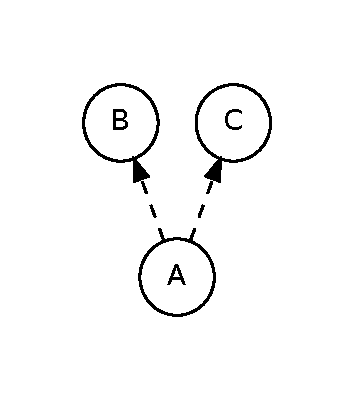
\includegraphics[scale=0.6]{figures/complementation/single-1.pdf}
    \subcaption{B and C must be subtype-related (in either
      direction).}\label{fig:single1}
  \end{minipage}
  \hspace{0.4in}
  \begin{minipage}[t]{0.5\linewidth}
    \centering
    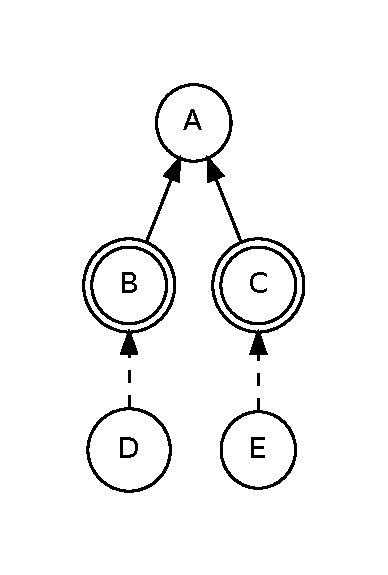
\includegraphics[scale=0.6]{figures/complementation/single-2.pdf}
    \subcaption{D and E cannot be subtype-related.}\label{fig:single2}
  \end{minipage}
  \\
  \begin{minipage}[t]{0.5\linewidth}
    \centering
    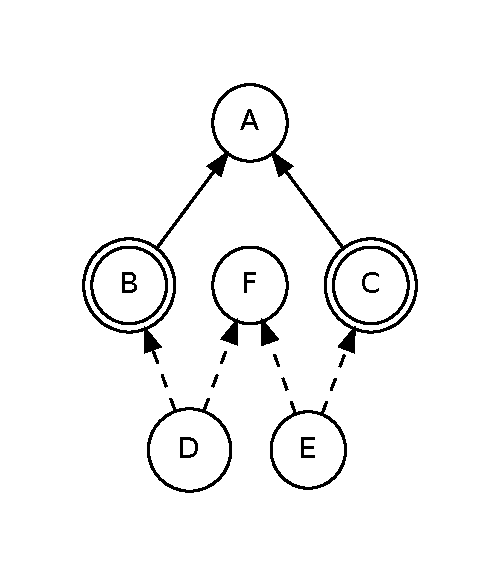
\includegraphics[scale=0.6]{figures/complementation/single-3.pdf}
    \subcaption{A has to be a subtype of F.}\label{fig:single3}
  \end{minipage}
  \hspace{0.2in}
  \begin{minipage}[t]{0.5\linewidth}
    \centering
    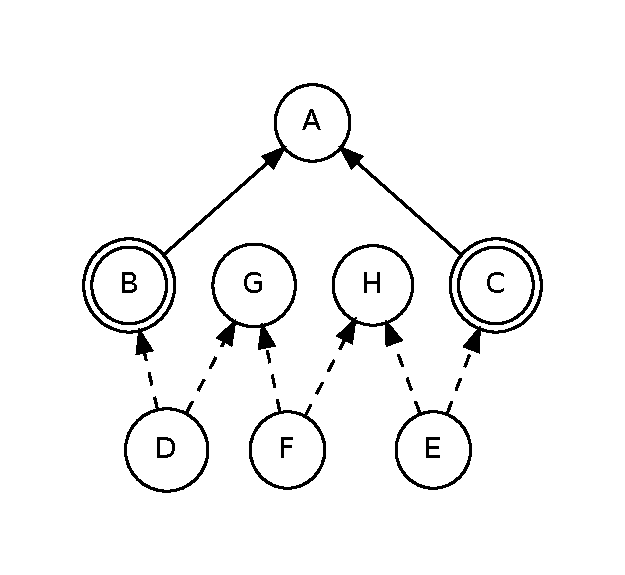
\includegraphics[scale=0.6]{figures/complementation/single-4.pdf}
    \subcaption{A has to be a subtype of either G or
      H.}\label{fig:single4}
  \end{minipage}
  \caption{Single Inheritance Basic Patterns}
\end{figure*}

Composing such constraints into more complex hierarchies gives an idea
of the difficulty of the search involved. Figure~\ref{fig:hard:or}
shows an example where it is hard to see without complex
reasoning which of the $E$, $F$, $G$ nodes have to be placed
above $A$ and which cannot.

\begin{figure}
  \centering
  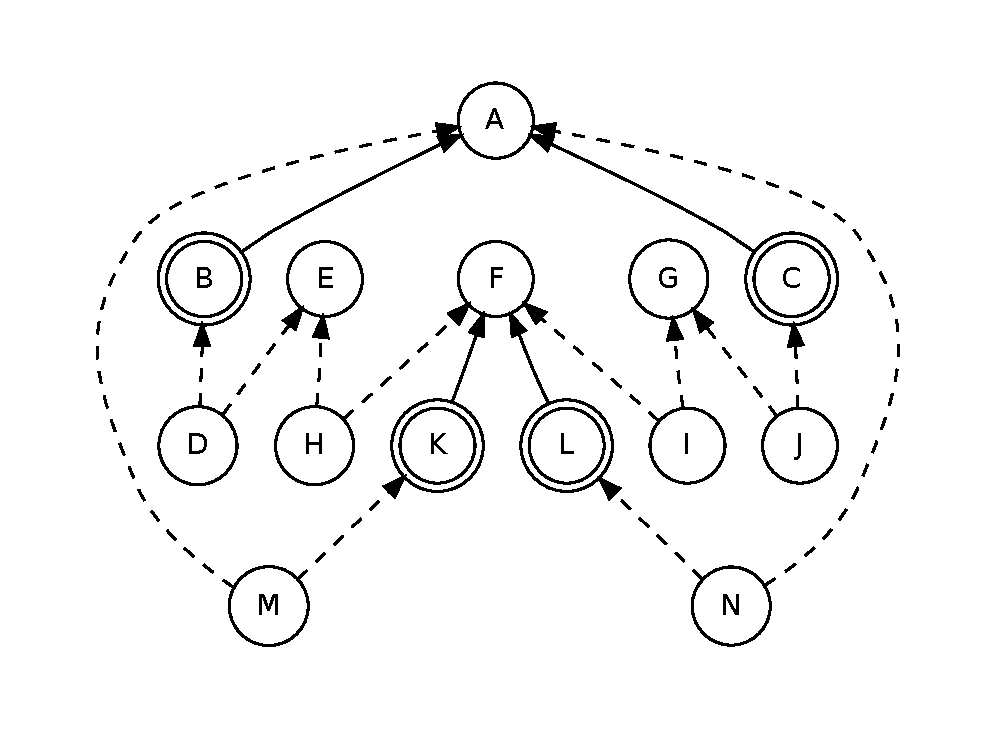
\includegraphics[scale=0.7]{figures/complementation/single-or.pdf}
  \caption[Harder composite example of single-inheritance
  constraints]{ Harder composite example of single-inheritance
    constraints.  The (undirected) path from $B$ to $C$ through
    $E,F,G$ implies that $(A <: E) \lor (A <: F) \lor (A <:
    G)$. However, since $F$ is the first common known supertype of $M$
    and $N$, and $A$ just a supertype of both, $F <: A$, and thus
    $(A <: E) \lor (A <: G)$. }
\label{fig:hard:or}
\end{figure}

%%You keep using that word, comprise. I don't think it means what you
%%think it means.

Clearly the problem can be modeled as a constraint satisfaction
problem instance, where $V_{phantom}$ is our set of variables and $V$
is the domain of values (representing the variable's direct
supertype). The path-edges and the absence of cycles constitute our
constraints. This requires an exponential search in the worst
case. Indeed, our implementation performs precisely such an exhaustive
search, but with a heuristic choice of nodes so that the search tries
to satisfy the constraints introduced by the patterns in
Figures~\ref{fig:single1} and \ref{fig:single2}---i.e., the pattern of
Figure~\ref{fig:single1} is identified, all induced permutations are
tried, and the pattern of Figure~\ref{fig:single2} is used to prune
them eagerly, instead of waiting to detect failure later.

Most importantly, our approach provides special handling for a
simple but practically quite common case. In this special case,
there is a polynomial algorithm for solving the problem and exhaustive
search is avoided.
%\footnote{More accurately, the special case algorithm
%is used as a subroutine and exhaustive search is performed by having
%the special case algorithm return different solutions when one fails.}

\begin{algorithm}[thp]
  \caption{Single-inheritance solver for strictly known direct-supertypes}
  \label{hiercomp/alg:single:kdirect}
  \small
  \hrulefill

  \begin{algorithmic}[1]
    \Function{solve}{$G = (V,E)$}
    \State{let $R$ be the ``\emph{root}'' node of $V$}
    \State{let $S$ be the tree of known nodes $(V_{known}, E_{direct})$}
    \ForAll{$(s,t) \in E_{path} : s \in V_{known}$}
      \If{$\nexists$ path $s \leadsto{} t$ in $S$}
        \State \Return error (unsatisfiable constraint)
      \EndIf
      \Let{$E_{path}$}{$E_{path} \setminus \{(s,t)\}$}
      \Comment{remove already satisfied edge}
    \EndFor
    \ForAll{$v \in V_{phantom}$}
      \State\Call{makeSet}{$v$}
      \Comment{create single-element disjoint sets}
    \EndFor
    \ForAll{$(s,t) \in E_{path} : t \in V_{phantom}$}
      \State\Call{union}{$s$, $t$}
      \Comment{merge two connected (phantom) components}
    \EndFor
    \Comment{result: undirected connected components (UCCs)}
    \ForAll{$v \in V_{phantom}$}
      \Let{$k$}{\Call{find}{$v$}}
      \Let{$\textit{top}[k]$}{$R$}
      \Comment{initially ``root''}
    \EndFor \Comment{init UCC's lowest common known superclass (LCS)}
    \ForAll{$(s,t) \in E_{path} : t \in V_{known}$} \Comment{must be $s \in V_{phantom}$}
      \Let{$k$}{\Call{find}{$s$}}
      \If{$\exists$ path $t \leadsto \textit{top}[k]$ in $S$}
        \Let{$\textit{top}[k]$}{$t$}
        \Comment{lower superclass found, update LCS}
      \ElsIf{$\nexists$ path $\textit{top}[k] \leadsto t$ in $S$}\label{hiercomp/lst:line:crossover}
        \State \Return error (unsatisfiable constraint)
      \EndIf
    \EndFor
    \ForAll{$k \mapsto v$ in \textit{top}}
    \Comment{for each UCC and its LCS}
      \Let{$U$}{$\{(s,t) \in E_{path} : t \in V_{phantom} \land \textsc{find}(s) = k\}$}

      \Comment{directed subgraph of original over nodes of this UCC}
      \Let{$L$}{a topological order of $U$}
      \Comment{linearize subgraph}
      %% \ForAll{$(x,y)$ in $zip(L,tail(L))$}
      %% \EndFor
      \Let{$hd$}{the top node of $L$}
      \Let{$S$}{$S \cup L \cup \{(hd,v)\}$} 
%      \While{$L$ is not empty}
%        \State $hd::L' = L$
%        \Comment{unpack head-tail of list $L$}
%        \Let{$S[hd]$}{$v$}
%        \Comment{set $v$ as the direct-supertype of $hd$ }
%        %% \Comment{set $v$ as the direct-supertype of $hd$}
%        %% \State add $(v,hd)$ to $S$
%        \Let{$v, L$}{$hd, L'$}
%        \Comment{advance $L$ and renew $v$}
%      \EndWhile
    \EndFor
    \State \Return{$S$}
    \EndFunction
  \end{algorithmic}
\end{algorithm} 



%%% Local Variables: 
%%% mode: latex
%%% TeX-master: "../../doc"
%%% End: 


\paragraph{Simplified setting: No direct-edges to phantom nodes.}

It is easy to solve the problem in the case that there are no direct
edges from known nodes to phantom nodes. Since we are in a
single-inheritance setting, this means that no class in the known part
of the program has a superclass in the complement that we are trying
to produce. In this case, we have that $E_{direct} \subseteq
V_{known}\times V_{known}$. The extra condition allows us to employ a
fast polynomial time algorithm. This interesting case of our problem
is very common in practice. Intuitively, the ease of dealing with this
case stems from avoiding the search in the space of permutations when
the input contains patterns such as those in Figure~\ref{fig:single3}:
if two permutations have elements in common (e.g., the permutation of
$B$ and $F$, and that of $F$ and $C$ in Figure~\ref{fig:single3}) they
cannot include nodes that are guaranteed to be subtype-unrelated (such
as $B$ and $C$ in this example) and all unknown nodes have to be below
the known ones in any solution.

Algorithm~\ref{alg:single:kdirect} first removes path-edges
originating from known-nodes, after verifying that the corresponding
paths indeed exist. It then uses union/find data structures to compute
connected components of phantom nodes, while treating path-edges
as \emph{undirected} edges: anything connected through such edges can
safely end up in a single linear ordering. Then, for each phantom
undirected connected component, it computes the lowest known-node to
serve as the first-common-supertype of all of this component's phantom
nodes. Note that when two known-nodes are reachable by two phantom
nodes of the same connected component (in the phantom subgraph), then
one of them ought to be a supertype of the other, or else no solution
can exist in a single inheritance setting. This condition is captured
in line~\ref{lst:line:crossover}. After the first common (known)
supertype for every connected component has been computed, a mere
topological sort, i.e. placing all relevant nodes in a total order, is
enough to satisfy all of this component's constraints. This may
introduce many superfluous edges in the solution: these edges are not
actually required by our constraints (since a topological order is a
total order). In practice, we produce a partial order by using a
variant of topological sort that generates a tree instead of a list as
its result, but a full topological sort also satisfies the correctness
requirements of the algorithm. (We return to the topic of why we
actually want a weaker ordering in Section~\ref{java}.)

In the example of Figure~\ref{fig:kdirect:ex},
Algorithm~\ref{alg:single:kdirect} first checks and removes the
$(F,A)$ path-edge. Then the phantom nodes are divided in the following
phantom connected components: $\{G,H,I\}$, $\{J,K,L\}$, and
$\{M\}$. The first common known supertype for each component is $B$,
$F$, and $F$ respectively. Each component is then linearized, which
generates the following complete orders that are appended to the
output: $I <: H <: G <: B$, $K <: J <: L <: F$, and $M <: F$.

% CHECK list of figure names

\begin{figure}[t]
  % \hspace{-6mm}
  \begin{minipage}[b]{.5\linewidth}
    \centering
    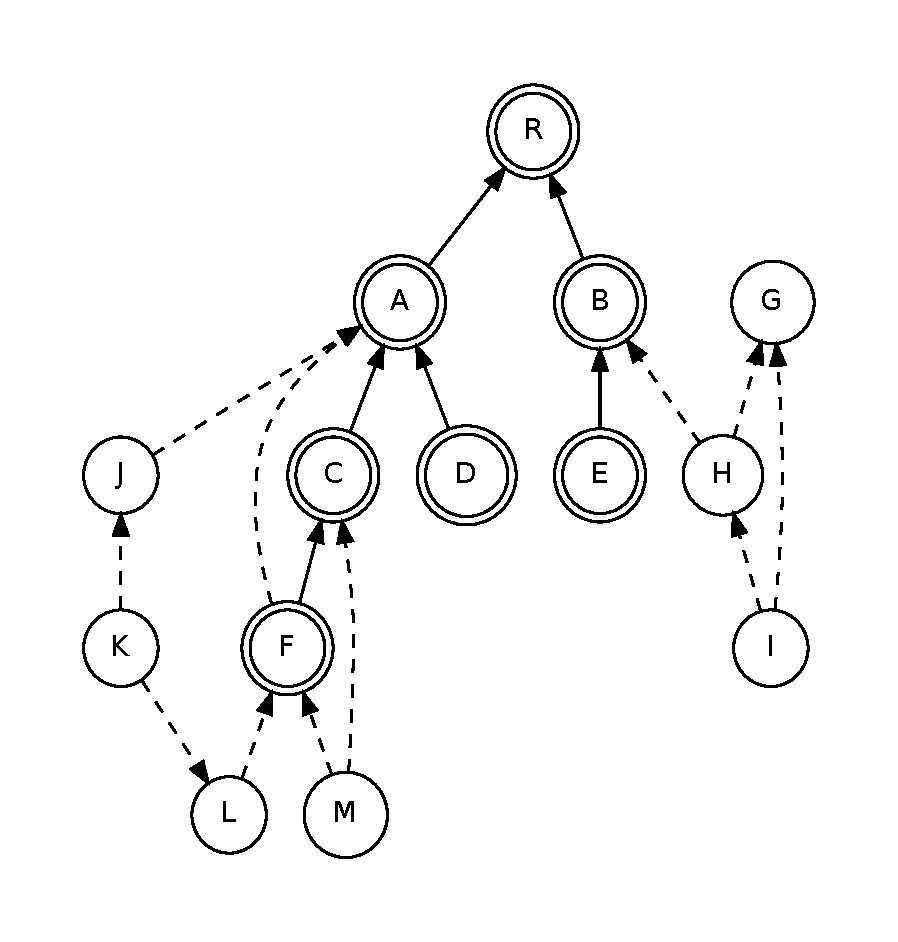
\includegraphics[scale=0.6]{figures/complementation/single-direct.pdf}
    \subcaption{Constraint Graph}\label{fig:stree1:simple}
  \end{minipage}
  % \hspace{-5mm}
  \begin{minipage}[b]{.5\linewidth}
    \centering
    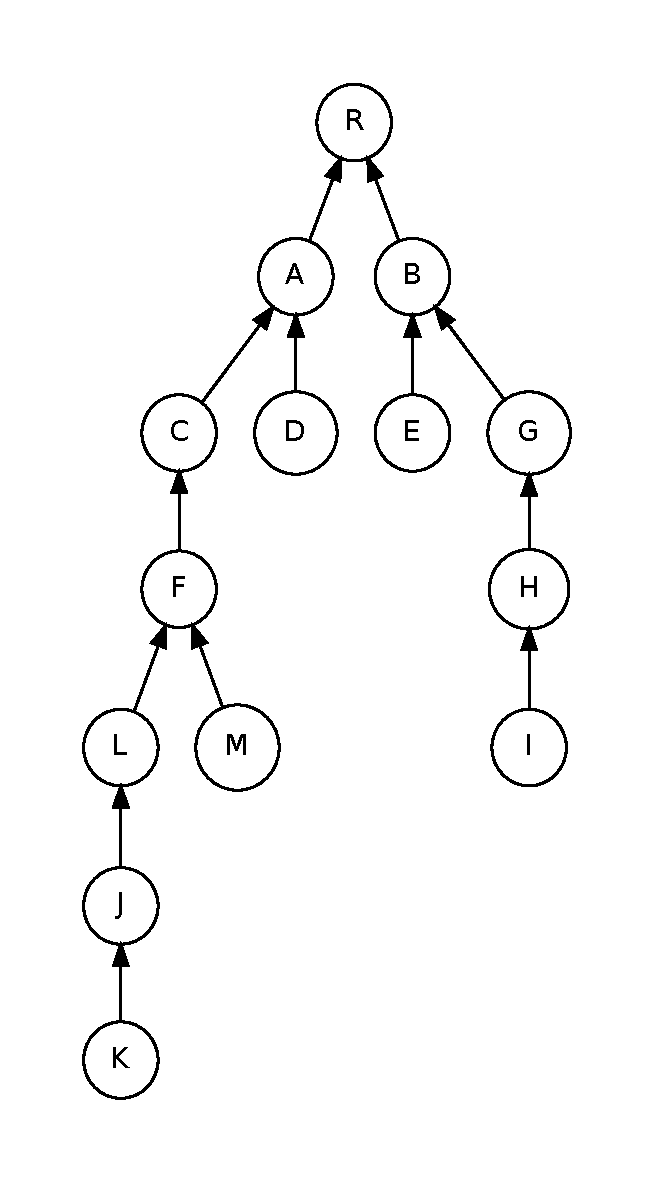
\includegraphics[scale=0.6]{figures/complementation/single-direct-sol.pdf}
    \subcaption{Solution}\label{fig:cgraph1:simple}
  \end{minipage}
  \caption[Single Inheritance Algorithm Example]{%
    Algorithm~\ref{alg:single:kdirect} - Example. }
  \label{fig:kdirect:ex}
\end{figure}

%% Do we care? Seems like a leftover.
%A phantom-only input, i.e. $V = V_{phantom}$, $E = E_{path}$, poses no
%difficulties in this setting too, since a single topological sort
%would suffice as an acceptable solution. (A solution, for our
%purposes, yields a correct program complement exactly when one exists,
%i.e., is both sound and complete.)



\begin{comment}
%%%%%%%%%%%%%%%%%%% Old stuff follow

However, in order to achieve a solution that generalizes well to
harder cases, we would like to avoid ordering nodes if there is no
need for them to be ordered. The result will be a tree and not a
linear order (in the general case). Specifically, we would like to
compute a partial order relation,\footnote{Throughout the paper, our
use of the term ``partial order'' denotes an irreflexive partial
order.} $\ll$, such that:

\begin{itemize}
\item $\ll$ subsumes the input constraints, i.e., $v_a \ll v_b$ if $(v_a,v_b) \in E$
\item if $v_c \ll v_a$ and $v_c \ll v_b$ then either $v_a \ll v_b$ or $v_b \ll v_a$
\item $\ll$ is transitively closed
\item $\ll$ is minimal, i.e., removing any pair from the relation would violate
the above rules.
\end{itemize}

The addition of the second rule, above, is a hallmark feature of the
hierarchy complementation problem. Consider the input of
Figure~\ref{fig:diamond}. The $(B,A)$ and $(C,A)$ edges guarantee that
both $B$ and $C$ will be ordered below $A$ in the result.  However, we
also know that they should be ordered relative to each other: the
$(D,B)$ and $(D,C)$ edges enforce this requirement, since there can
only be a single path from $D$ to the root of the hierarchy and both
$B$ and $C$ must be on it. Note that, in the absence of
other ordering constraints, we could have either $B \ll C$ or
$C \ll B$---both options would yield $\ll$ relations that satisfy the
above requirements, for this example.

%% \begin{defn}
%%   A solution $G_S = (V,E')$ to a set of subtype constraints $G_C =
%%   (V,E)$ is minimum if and only if, $\forall x,y \in V$ such that a
%%   path $p = x \ldots y$ exists in $G_S \Rightarrow$ .
%% \end{defn}

\begin{figure}
  \centering \includegraphics[width=0.2\textwidth]{images/diamond.pdf}

  \caption{In any solution of these subtyping constraints, B and C
  have to be below A, but also they have to be relatively ordered with
  each other, since D must find both on its (single inheritance) path
  to the root.}
\label{fig:diamond}
\end{figure}

Algorithm~\ref{alg:single:simple} produces an ordering relation
(represented as a ``solution'' set of ``direct parent'' edges, $S$)
whose transitive closure satisfies the requirements for
$\ll$,\footnote{I.e., the algorithm computes the \emph{transitive
reduction} of $\ll$, or, in diagram form, the Hasse diagram of the
$\ll$ partial order, i.e., the depiction of the partial order with
direct-predecessor-only edges.} or signals an error if none
exists. The algorithm is given in pseudocode, mixed with informal
well-understood operations when their precise description would be
tedious. Such concepts include ``remove vertex and all incoming
edges'', ``undirected view of a directed graph'', ``maximally
connected component'', ``restriction of a graph to a subset of its
nodes''.

Function \textsc{placeUnder()} augments the solution being generated
by placing every node of its first argument, graph $G$, under its
second argument, node $n$. The invariant maintained across recursive
invocations is that, on entry, $n$ is a node of $G$ with no outgoing
edges and all nodes of $G$ can reach $n$ \emph{when the edges of G are
converted to undirected edges}.  The key to the algorithm is precisely
this property: we order below a node all other nodes that can reach it
with edges considered in any direction, thus satisfying the properties
of the $\ll$ definition. A key lemma (proven by induction) is that if
an unconstrained node (i.e., one without outgoing edges), $u$, can
reach another node, $k$, via any combination of up-or-down subtyping
inferences, then $u$ and $k$ have a common descendant, i.e., a node
that has (directed) paths to both. Therefore $u$ and $k$ must be
relatively ordered (although it is not known in which direction).  By
also picking to place a subtree under one of its nodes with no
outgoing edges (mimicking a plain topological sort), we ensure that
the arbitrary ordering picked (to satisfy the second rule of the $\ll$
definition) does not violate explicit ordering constraints in the
input (per the first rule of the $\ll$ definition). The above
properties also serve as a proof sketch for the correctness of
Algorithm~\ref{alg:single:simple} relative to the definition of $\ll$.

% Thus, to create our solution, given that our
%constraint graph is weakly connected---and if it's not, we can make it
%so by adding auxiliary edges to the \emph{root} node---we only have to
%call \textsc{placeUnder()} with the \emph{root} node as its second
%argument.

\begin{algorithm} 
  \caption{Single-inheritance phantom-only solver}
  \label{alg:single:simple}
  \hrulefill

  \begin{algorithmic}[1]
    \Function{solve}{$G = (V,E)$}
    \State{let $v_r$ be the ``\emph{root}'' node of $V$}
    \State \Return \Call{placeUnder}{$G$, $v_r$}
    \EndFunction
  \end{algorithmic}

  \hrulefill

  \begin{algorithmic}[1]
    \Function{placeUnder}{$G = (V,E)$, $n$}
       %% \Comment $G_u$ reflects changes in $G$
       \Let{$S$}{$\emptyset$}
       \State remove vertex $n$ (and its incoming edges) from $G$ 
       \Let{$V_n$}{$\left\{ x \in V : \not \exists (x,y) \in E \right\}$} \Comment all nodes with no outgoing edges
       %% \Comment unconstrained nodes
       %% \State $UV \gets V \setminus \left\{ x : (x,y) \in E
       %% \right\}$
       \While{$V_n \neq \emptyset$} 
          \State $x \gets$ \Call{pick}{$V_n$, $n$}
          \State $V_n \gets V_n \setminus \left\{x\right\}$ 
          \If{$x \in V$} \Comment otherwise it has been ordered by earlier iteration
             \Let{$S$}{$S \cup \{(x,n)\}$} \Comment add edge $(x,n)$ to solution
             %% \Comment $x$ extends $n$
             \State let $G_u$ be the undirected view of $G$ 
             \State let $V'$ be the nodes of the maximally connected 
               component of $G_u$ that contains $x$
             \State let $G' = (V',E')$ be the restriction of $G$ to $V'$ \Comment Note: $G'$ is directed
             \State $G \gets (V \setminus V', E \setminus E')$ \Comment remove from $G$ all nodes in $V'$ and adjacent edges
%             \ForAll{$v \in V'$}
%             \State remove $v$ and its adjacent edges from $G$
%             \EndFor
%             \Let{$S_x$}{\Call{placeUnder}{$G' = (V',E')$, $x$}} \Comment recurse for the removed subgraph
             \Let{$S$}{$S \cup $ \Call{placeUnder}{$G' = (V',E')$, $x$}} \\
                               \Comment recurse for removed subgraph, accumulate solution edges
          \EndIf
       \EndWhile
       \If{$G$ has edges} \Comment all nodes have outgoing edge (cycle)
         \State error: no solution  \label{lst:line:cycle}  %(graph has at least one cycle)
       \EndIf
       \State \Return $S$
    \EndFunction
  \end{algorithmic}

  \hrulefill

  \begin{algorithmic}[1]
    \Function{pick}{$V$, $n$}
    \State \Return random element of $V$
    \EndFunction
  \end{algorithmic}
\end{algorithm} 



An example is given in Figure~\ref{fig:ex1:simple}. We assume that
node $A$ is the \emph{root} node. Therefore, the algorithm will first
call \textsc{placeUnder($G_C$, $A$)} and then erase the edges
$\{(B,A), (C,A), (D,A), (E,A), (I,A)\}$. The set of unconstrained
nodes, $V_n$, will contain the nodes $B,C,E$. Without loss of
generality, we assume that the \textsc{pick()} function always returns
the lexicographically smaller node of its candidates. Thus, the edge
$(B,A)$ is added to the solution, and \textsc{placeUnder()} is
recursively called for the component of $G$ that contains only the
edge $(D,B)$, which is then also removed from $G$ and added to the
solution. The control flow will go back to node $A$, pick the next
unconstrained node, $C$, and call \textsc{placeUnder()} again after
adding the edge $(C,A)$ to the solution. This time, the component
computed (by undirected reachability) to be under $C$ will contain
every remaining node, and will therefore prevent any other node from
being placed directly under $A$. After edge $(F,C)$ is removed, the
unconstrained nodes now become $E$ and $F$. The edge $(E,C)$ is added
and $(G,E),(H,E)$ are removed. Again, every remaining node will be
placed under $E$. The node $F$ is picked among $F,G,H$, edge $(F,E)$
is added, and $G'$ gets every remaining edge except $(H,E)$ because
$H$ is (undirected-)unreachable by $F$. Edge $(H,E)$ will be added
eventually, after $G,J,I$ have been recursively placed under $F$ in
this order.

\begin{figure}
  \centering
  \subfloat[Constraint Graph]{
    \includegraphics[scale=0.4]{images/cgraph1.pdf}
    \label{fig:stree1:simple}
  }
  \subfloat[Solution]{
    \includegraphics[scale=0.4]{images/stree1.pdf}
    \label{fig:cgraph1:simple}
  }
  \caption{%
    Algorithm~\ref{alg:single:simple} - Example
  }
\label{fig:ex1:simple}
\end{figure}



%
%We can then decouple the two different types of edges into the $f_i$
%mapping and a graph $G_C = (V,E_{path})$. For ease of notation, we
%will use $f_i$ and $G_C = (V,E)$ from now on, as a shorthand, but each
%edge of $G_C$ will represent a path-edge: $\forall (x_1,x_n) \in
%E : \text{there exists a path } (x_1,x_2,\ldots, x_n) \text{ in } G_T$.
%
%
%Let us ignore, for now, the subset of fixed edges that corresponds to
%$f_i$ and should eventually be present in any solution. This variation
%of our problem means that we allow only phantom types in our
%constraints, for which no supertype information exists, whatsoever. A
%simple solution to this problem would be a topological order
%w.r.t. our constraints $E$.


\paragraph{Full single inheritance setting: known and phantom nodes.}

We can extend our algorithm to support an existing class hierarchy by
combining a simple preprocessing step and a biasing of
function \textsc{pick} so that it preferentially returns a direct
child, if one exists in the input. Recall that our input is now two
distinguished sets of nodes, $V_{known}$, $V_{phantom}$ and similarly
for edges, $E_{direct}$, $E_{path}$.  For notational convenience we
represent $E_{direct}$ as a function $f_i:V_{known} \rightarrow
V$. (Since we are in a single inheritance setting, we can guarantee
that $E_{direct}$ is a function from its first argument: if a node
$v \in V_{known}$ has more than one outgoing edge then the problem is
immediately unsolvable. Our solution edge set is similarly a function,
since we are computing a tree.)


%Similarly, since $G_T$ has to be a tree, we can also encode our
%solution (output) as another mapping, $f_o:V \rightarrow V$.  Both of
%these mappings map a type (key) to its \emph{direct}-supertype
%(value). Thus, the first constraint of our solution becomes: $\forall
%v \in V_{known} : f_o[v] = f_i[v]$, where $f_i[v]$ denotes the known
%direct supertype of $v$ (given as input), and $f_i$ can now be viewed
%as a partial solution that should be preserved by our final solution
%$f_o$.

The preprocessing step consists of merely adding subtyping edges from
all known supertypes of a type to all its unknown ones. In other
words, the principle is that if a node $n$ can reach another node $m$
through a path of $E_{direct}$ edges, while $n$ reaches $m'$ via an
$E_{path}$ edge, then the solution should have a path from $m$ to
$m'$.  By transitively following the $f_i$ function (i.e.,
$E_{direct}$ edges) we can add outgoing edges to all nodes found on
this path, so they will never be placed above a node ordered relative
to their descendant via $E_{path}$, thus violating the requirement of
preserving the input hierarchy. This is shown in
Algorithm~\ref{alg:single:ext}. Function \textsc{solve()} performs
the preprocessing step while keeping the core logic, i.e. the earlier
\textsc{placeUnder()} function, intact. Function \textsc{pick()}
prioritizes known direct descendants, in order to maintain the
$E_{direct}$ edges in the output.

\begin{algorithm} 
  \caption{Single-inheritance extended solver}
  \label{hiercomp/alg:single:ext}

  \hrulefill

  \begin{algorithmic}[1]
    \Function{solve}{$G = (V,E)$}
     where $V = V_{known} \cup V_{phantom}$ and $E = E_{direct} \cup E_{path}$
    \State \Global $f_i$ \Comment global var as convenience, to keep same args for \textsc{placeUnder}, \textsc{pick}
    \ForAll{$(v_s,v_t) \in E_{direct}$}
      \If{$\exists (v_s, v_{t'}) \in E_{direct}$ such that $v_t \neq v_{t'}$}
        \State error: input not a tree
      \Else
        \Let{$f_i[v_s]$}{$v_t$}
      \EndIf
    \EndFor
%    \ForAll{$c \in V_{known}$}
      %% \State add edge $(c,f_i[c])$ to $E$ \label{hiercomp/lst:line:direct}
      \ForAll{$(c,c_s) \in E_{path}$}
        \While{$f_i[c] = p$} \Comment while there exists a known parent, which we shall call $p$
          \If{$p \neq c_s$}  \Comment just for tolerating extraneous path edges in input
            \State $E \gets E \cup
            \left\{(p,c_s)\right\}$ \label{hiercomp/lst:line:add}
            \Comment no need to update $E_{path}$, \textsc{placeUnder} only uses $E$
% $E$ add edge $(p,c_s)$ to $E$ \label{hiercomp/lst:line:indirect}
          \EndIf
          \Let{$c$}{$p$}
%          \Let{$c$}{$f_i[c]$}
        \EndWhile
      \EndFor
%    \EndFor
    \State{let $v_r$ be the ``\emph{root}'' node of $G$}
    \State \Return \Call{placeUnder}{$G$, $v_r$} \Comment{\textsc{placeUnder} treats direct and path edges the same}
    \EndFunction
  \end{algorithmic}

  \hrulefill

  \begin{algorithmic}[1]
    \Function{pick}{$V$, $n$}
    \If{$\exists v \in V: f_i[v] = m$} \label{hiercomp/lst:line:priority}
      \If{$n \neq m$}
        \State error: crossover %% \label{hiercomp/lst:line:crossover}
      \Else
        \State \Return $v$
      \EndIf
    \Else
    \State \Return random element of $V$
    \EndIf
    \EndFunction
  \end{algorithmic}
\end{algorithm} 



For example, in Figure~\ref{fig:ex1:ext} we can see how the solution
of Figure~\ref{fig:ex1:simple} is altered if we take a given class
hierarchy into account. Let $V_{known} = \{F,J\}$ and $E_{direct}
= \{(F,C),(J,F)\}$. The solid edges denote the constraints added due
to $f_i$, while the newly added edges $(F,G),(C,G)$ have been inserted
because of $(J,G)$. Since $G$ is surely a supertype of $J$ and we know
that $F$ is the direct supertype, we can soundly add the edge $(F,G)$
to preserve their respective order. After $(F,G)$ has been added, and
because $f_i[F] = C$, we can soundly add $(C,G)$ and then reach a
fixpoint.

% (line~\ref{lst:line:indirect}).

Line~\ref{lst:line:priority} in the \textsc{pick()} function will
choose a \emph{direct} subtype according to $f_i$, over any other
unconstrained node. For instance, if ``$f_i[C] = A$'' were part of the
input in the earlier pattern of Figure~\ref{fig:diamond}, then
the \textsc{pick()} function would choose node $C$ among $V = \{B,C\}$
to place next, resulting in the $A \leftarrow C \leftarrow
B \leftarrow D$ ordering (and not $A \leftarrow B \leftarrow
C \leftarrow D$, as produced by settling arbitrary node choices according
to lexicographic order).

In line \ref{lst:line:crossover} of the \textsc{pick()} function, an
error is raised if a known direct supertype disagrees with what
we have computed. This can only happen if two subtrees of $G$ have
roots in $V_{known}$, and these two subtrees are somehow connected. In
this case, the problem is unsolvable for single
inheritance. An example would be the pattern of Figure~\ref{fig:diamond} if
$V_{known} = \{A,B,C\}$ and $E_{direct} = \{(B,A), (C,A)\}$. Our
algorithm would reach a point where either node $C$ would have to be
placed under $B$, or node $B$ under $C$. In both cases, this would
conflict with $f_i$, and would be captured by our
\emph{crossover} error check.

\begin{figure}
  \centering
  \subfloat[Constraint Graph]{
    \includegraphics[scale=0.4]{images/cgraph1-ext.pdf}
    \label{fig:stree1}
  }
  \subfloat[Solution]{
    \includegraphics[scale=0.4]{images/stree1-ext.pdf}
    \label{fig:cgraph1:ext}
  }
  \caption{%
    Algorithm~\ref{alg:single:ext} - Example
  }
\label{fig:ex1:ext}
\end{figure}

\paragraph{Correctness Proof Sketch:}

Algorithm~\ref{alg:single:simple} already satisfies all path-edge
constraints. The extended version (\ref{alg:single:ext}) adds new
path-edges soundly, i.e. an edge $(s,t)$ is added exactly when
$s$ \emph{has} to be a subtype of $t$. Therefore, to prove that our
algorithm is correct we only have to show that it maintains in the
output the direct-edges of its input.

The edges added by line~\ref{lst:line:add} of the \textsc{solve()}
function ensure that a node $k \in V_{known}$ will be placed in an
unconstrained set (i.e., $k$ has no outgoing edges) \emph{for the
first time} when the second argument of \textsc{placeUnder()} is equal
to its actual direct supertype: each direct supertype acquires edges
to all indirect, so that it becomes free of outgoing edges only after
each indirect supertype has been placed above it in the solution
hierarchy.

However, the phantom-only version of our algorithm guarantees that the
subset of nodes that will be placed underneath each unconstrained node
$u$ will only involve nodes that are somehow connected with $u$ at
that time.  Thus, if a known node $k$ were to be placed somewhere
lower than its direct supertype, there has to be another unconstrained
node $u$ to be placed above $k$ and $u$'s (undirected)-connected
component includes an edge to $k$, so that $k$ is included in
the \textsc{placeUnder} graph argument for $u$. However, since
the \textsc{pick()} function prioritizes known nodes over phantom
ones, $u$ can only be a known node that happened to be picked before
$k$ in the same unconstrained set (when both $u,k$ were to be placed
under their direct-supertype). This, however, is an unsatisfiable
condition upon which our algorithm signals an error. To see that the
error truly indicates unsatisfiability of the input, recall the
property of Algorithm~\ref{alg:single:simple} mentioned earlier: if a
node with no outgoing edges can reach another node through an
undirected path, then both nodes have a common descendant, i.e., a
node that can reach both through \emph{directed} paths, and thus they
should be ordered relative to each other. But this is impossible since
both nodes are known and both their direct supertypes and all their
supertypes have been ordered in the output (the supertype of one
should have the other node above it). Therefore, our algorithm fails
to compute a solution only when no valid solution according to our
formal criteria exists. Moreover, each solution it generates is sound
w.r.t. our constraint edges (both path and direct).


\end{comment}


%-------------------------------------------------------------------------------
% Single Inheritance, Multiple Subtyping
%-------------------------------------------------------------------------------

\section{Single Inheritance, Multiple Subtyping: Classes and Interfaces}
\label{java}

It is easy to combine the single- and multiple-inheritance
approaches of the last two sections in the context of a language that
has single inheritance but multiple subtyping.  It is a common case
for strongly-typed languages to allow multiple inheritance only for a
subset of types.
%, which are mostly used to denote structural conformance, instead of
%providing an actual implementation.
Java and C\#
interfaces \cite{Gosling:2005:JLS:1036643,Hejlsberg:2003:CLS:861332},
and Scala traits \cite{scala-overview-tech-report} are such examples.

In order to support such a separation, we have to introduce a new
dimension to our problem that can be simulated as a graph coloring
variant. Each node in $V$ can be assigned a color denoting its
inheritance type. A \emph{black} node can have many direct supertypes
(i.e., multiple inheritance), while a \emph{white} node can only have
one (i.e., single inheritance). We will use the terms ``white node''
(resp.~``black node'') and ``class'' (resp.~``interface'')
interchangeably.

Note that, initially, our input may not fully determine the final
color for each of its types. Thus, we have to introduce a new color
(\emph{grey}) to refer to the subset of nodes whose color is yet
undetermined. In the end, our solution should soundly determine a safe
color (black or white) for each of the (grey) input nodes, so that no
constraints of the verifier will be violated.

Therefore, our solution in this new setting is a synthesis of a single
inheritance and a multiple inheritance solution. That is, the output
of our algorithm should be a \emph{DAG} that satisfies the same
conditions as those in the multiple inheritance setting, $G_S =
(V,E')$, and a function $f_c:V \rightarrow \{black, white\}$, such
that the restriction of $G_S$ to $\{v \in V: f_c(v) = white\}$ (i.e.,
white nodes) is a tree.

To safely decompose our problem into two different subproblems (one
for single and one for multiple inheritance), we assign colors to all
nodes as a preprocessing step. There are two kinds of constraints that
lead to restricting the colors of a node. First, we have local
constraints: we may get a node color from the initial input---i.e., an
observed bytecode instruction (such as \code{invokeinterface}) may
directly restrict the color of a phantom type. (More constraints of
this form are discussed in Section~\ref{jphantom}.) Second, we may get
transitive constraints, due to restrictions on subtyping. Interfaces
can only subtype interfaces (except for the \code{Object} class in
Java). This leads to two types of transitive constraints: If a black
node $s$ has a path to node $t$, then $t$ must also be black
(interfaces can only extend interfaces). Symmetrically, if a node $s$
has a path to a white node $t$, then $s$ must also be white (classes
can only be extended by other classes).

%% Old text. I don't think it applies any more.
%Based on the above, the observation that leads to a safe decomposition
%of the coloring from the subsequent solving is the following: only
%phantom nodes whose incoming edges are all path edges can have their
%colors determined transitively. (A phantom node with a known direct
%subtype takes its color locally, from the kind of subtyping declared.)
%By examining all algorithms in our earlier sections we see that no
%extra edges are added to phantom nodes with only path edges
%incoming. Therefore, executing any of our solvers for the hierarchy
%complementation problem will not affect the coloring of any type
%relative to the coloring constraints of the original input.

% The only interaction of this logic with the algorithms of the previous
% sections is in case the solution creates paths that did not exist in
% the original inputs. Our multiple inheritance algorithm never does so.
% The single inheritance algorithm can also avoid introducing paths
% between previously unreachable nodes if we use a weaker ordering
% (producing a tree and not a linear list) in place of the topological
% sort step of Algorithm~\ref{alg:single:kdirect}. Such a sort makes two
% nodes ordered only if there was a path between them in the original
% input. The algorithm is straightforward but tedious and we elide it
% for lack of space.
% %% REVIEW! We need to think about this.

%For instance, for the input of Figure~\ref{fig:kdirect:ex}

Furthermore, phantom nodes with no color constraints can be safely
assumed to be interfaces (black), for maximum flexibility in solving
other constraints. It is always easier to satisfy a given set
of constraints in a multiple inheritance setting instead of a single
inheritance setting, since the conditions of single inheritance are
stricter (a tree is a DAG).

As a result of the above observations, we can color all nodes by
applying local or transitive constraints to the original input before
solving a single and a multiple inheritance hierarchy complementation
problem separately.  That is, we can follow every possible path from
any node whose color has already been set and mark the nodes we find
along the way accordingly. The color of our source node determines the
direction of movement (i.e., from white source nodes, we have to go
backwards). When this process is over, we can assign the color black
to all remaining undetermined (in terms of color) nodes.  An example
of this process can be seen in our earlier
Figure~\ref{fig:real-example}. Once we have assigned a
\emph{black-or-white} color to every node, we can split our constraint
graph into two subgraphs by isolating white-to-white edges (and
feeding them to a single inheritance solver). After we have determined
our class hierarchy, we can proceed with satisfying the rest of the
edges using multiple inheritance rules.

The key to this approach is that the single inheritance solver does
not need the output of the multiple inheritance solver to compute a
solution, and vice versa. All we need to ensure (for the multiple
inheritance solver) is that we take into account class supertypes that
are reachable through direct edges of a known class when determining
the class's \emph{projection set}. Thus, the class/interface
decomposition indeed produces two independent subproblems that can be
solved separately. The composition of the two solutions will certainly
not create any cycles, if its two subparts do not contain any. If that
was not the case, then there would be a cycle that contained at least
one class and one interface, which is impossible since no interface
can be a subtype of a class (other than \code{Object}) in Java.

As for our arbitrary choice of defaulting undetermined nodes to
interfaces, suppose that a solution exists if a subset $U$ of those
undetermined nodes were treated as classes. We could then transform
this solution to another one where these nodes were interfaces
instead. The single inheritance solution could be produced by
replacing each node in $U$ with its parent (in the former single
inheritance solution), w.r.t. its incoming edges, and then removing
it, until no nodes in $U$ were present. This process would still
satisfy all constraints on the remaining class nodes. A multiple
inheritance solution also exists. Consider the union of the former
multiple plus single inheritance solution. The result is a DAG that
respects all of the multiple inheritance setting constraints. Again,
we can erase any edges to class-determined nodes (i.e., all class nodes
that are not in $U$) in a way that all subtype relations involving the
rest of the nodes remain unaltered, i.e., by iteratively replacing an
edge to a class-determined node with edges to all of its direct
supertypes, until no edges to class-determined nodes are left. This
process would yield a valid multiple inheritance solution that can be
safely combined with the single inheritance one. Therefore, marking
undetermined nodes as interfaces does not affect the outcome of our
algorithm, i.e., no solution will be found if and only if no solution
existed.


% A single inheritance solution for the class subset would
% still exist (since removing some nodes from a tree---representing the
% former single inheritance solution---by replacing them with their
% parent (w.r.t adjacent edges) satisfies all constraints on the
% remaining nodes). A multiple inheritance solution also exists.
% Consider the union of the former multiple inheritance solution and the
% relevant part of the former single inheritance solution that contains
% exactly these undetermined nodes and their adjacent edges. The result
% is a DAG that respects all of the multiple inheritance setting
% constraints. Again, we can erase any edges to class-determined nodes
% in a way that all subtype relations involving the rest of the nodes
% remain unaltered, i.e. by iteratively replacing an edge to a
% class-determined node with edges to all of its direct supertypes until
% no edges to class-determined nodes are left. The outcome will be a
% valid multiple inheritance solution that can be safely combined with
% the single inheritance one.


%-------------------------------------------------------------------------------
% Implementation and Evaluation
%-------------------------------------------------------------------------------

\section{Implementation and Practical Evaluation}
\label{jphantom}

We next discuss practical aspects of our implementation. First, we
consider the \emph{program analysis} part of our work, which solves
the problem of producing complements of a partial Java program by
appealing to the solver of the class hierarchy complementation
problem. Subsequently, we present experiments applying our JPhantom
tool to real programs.

\subsection{JPhantom Implementation}

JPhantom is a practical and scalable tool for program complementation,
based on the algorithms we have presented in this
paper. \footnote{JPhantom is available online at
  \url{https://github.com/gbalats/jphantom}.} JPhantom uses the ASM
library~\cite{Bruneton02asm:a} to read and trasform Java
bytecode. Given a jar file that contains phantom references, it
produces a new jar file with dummy implementations for each phantom
class. The resulting jar file satisfies all formal constraints of the
JVM Specification \cite{Lindholm:1999:JVM:553607}. We
give a brief explanation of the different stages of computation for
the analysis of an input jar file by JPhantom.

%% LaTeX sucks when deciding placement of single-column figures in
%% two-column mode. We have to manually place the figure below.

\begin{figure}[thp]
\centering
\small
\begin{savenotes}
\renewcommand{\arraystretch}{1.3}
\begin{tabular}{@{}>{\footnotesize\ttfamily}l@{\hspace{1em}}l@{\hspace{1em}}l@{\hspace{1em}}l@{}}
  \toprule
  \normalfont{\small\emph{Opcode}}
                  & \emph{Types}
                  & \emph{Stack Types}
                  & \emph{Constraints} \\
  \hline
  AASTORE         &
                  & $a:E[] \: \; i:int \; \: v:V$
                  & $V <: E$
  \\
  ARETURN         &
                  & $\textit{obj}:S$
                  & $S <:R_m$
  \\
  ASTORE          & $T$
                  & $\textit{obj}:S$
                  & $S <: T$
  \\
  ATHROW          &
                  & $\textit{obj}:S$
                  & $S <:$ ``\code{java.lang.Throwable}''
  \\
  GETFIELD        & $T.F$
                  & $\textit{obj}:S$
                  & $\textit{isClass}(T) \land S <: T$
  \\
  PUTFIELD        & $T.F$
                  & $\textit{obj}:S \; \: v:U$
                  & $\textit{isClass}(T) \land S <:T \land U <: F$
  \\
  PUTSTATIC       & $T.F$
                  & $v:U$
                  & $\textit{isClass}(T) \land U <: F$
  \\
  INVOKEINTERFACE & $T.(\overline{A})R$
                  & $\textit{arg}_0:S_0 \;\: \textit{arg}_1:S_1$ \ldots
                  & $\textit{isIface}(T) \land S_0 <: T$
  \\
  INVOKEVIRTUAL   & $T.(\overline{A})R$
                  & $\textit{arg}_0:S_0 \;\: \textit{arg}_1:S_1$ \ldots
                  & $\textit{isClass}(T) \land S_0 <: T$
  \\
  INVOKESPECIAL   & $T.(\overline{A})R$
                  & $\textit{arg}_0:S_0 \;\: \textit{arg}_1:S_1$ \ldots
                  & $\textit{name} =$ ``\code{<init>}'' $\Rightarrow \textit{isClass}(T) \land S_0 <: T$
  \\
  INVOKESTATIC    & $T.(\overline{A})R$
                  & $\textit{arg}_1:S_1$ \ldots
                  & $\textit{isClass}(T)$
  \\
  INVOKE*         & $T.(\overline{A})R$
                  & $(\textit{arg}_0:S_0) \;\: \textit{arg}_1:S_1$ \ldots
                  & $S_i <: A_i, \forall i=1,...$
  \\
  \bottomrule
\end{tabular}
\end{savenotes}
\caption[Generated Bytecode Constraints]{%
    \emph{Generated Bytecode Constraints}. At this point, our analyzer has
    already computed the (sets of) types for every stack and local
    variable at every point of execution (bytecode in method). For
    simplicity, we assume that each set of reference types contains a
    single element (3rd column). Each bytecode may involve some
    declared types (2nd column) by references in the constant pool or
    by entries in the local variable table (if such exists). Also, let
    $R_m$ be the containing method's return type.
}
\label{fig:constraints}
\end{figure}

%% Is this a leftover???
%\footnotetext{$<$clinit$>$ is never called explicitly}

JPhantom execution consists of the following steps. It (1) performs a
first pass over the jar contents in order to recreate the existing
class hierarchy (type signatures only) and store the field and method
declarations of the contained classes, then (2) makes a second pass to
extract all phantom references and store the full class
representations. A third pass (3) extracts all relevant type
constraints, before (4) they are fed to JPhantom's hierarchy
complementation solver, which computes a valid solution, if such a
solution is possible. At this point, we can proceed to (5) bytecode
generation, where we create new class files for our missing (phantom)
types. Finally, we compute method bodies to add to each type. For
instance, when the solver determines that a phantom-class type $X$
must implement an interface type $Y$, all missing methods of $Y$
should be added to $X$, so that the resulting bytecode is valid. After
all such methods have been computed, they are added in the last (6)
step of execution.

Phantom references include references to missing classes, as well as
references to missing fields and methods. Note that both phantom and
existing classes may have references to missing members, since there
are cases of existing classes calling a method or referencing a field
declared in one of their phantom supertypes. JPhantom detects all such
references and adds the relevant missing declarations to its
output. If a member is missing from a phantom class, we add it
directly to that class as part of JPhantom's output. Otherwise, if a
member is missing from an existing class, we add it to an appropriate
phantom supertype in its projection set instead. We encode these
declarations as additional constraints over the missing classes,
generated in the second step of JPhantom's execution. It suffices to
use the existing class hierarchy and declared members (step 1), to
perform member lookup for the purpose of determining if a member is
missing and where it should be added.

The most interesting aspects of the above steps have to do with
analyzing the bytecode to produce the constraints (step 3) used as
input to the hierarchy complementation algorithm. In order to extract
type constraints, we have to simulate a symbolic execution of Java
bytecode by following every possible execution path, while computing
the types of stack and local variables. This is necessary because, in
general, bytecodes receive some untyped arguments whose types we need
to infer, in order to extract our constraints. This process is
analogous to Pass~3
\cite[Section~4.9.2]{Lindholm:1999:JVM:553607} of the bytecode
verification process.

When computing such type information for stack and local variables,
there are points where we have to merge two different paths of
execution. That is, the two paths may map the same variable to
different types, in which case we have to merge two different types
into a new one. Typically, when merging two types $A,B$ the resulting
type is the first common superclass of $A$ and $B$. In Java, there
always exists such a common superclass since every reference type
(interfaces included) is a subtype of \code{java.lang.Object}.

In our case, however, since we do not have the complete type hierarchy
at the time of constraint extraction, we cannot compute the first
common superclass for any two nodes. This is why we apply the
alternative technique of storing \emph{sets of reference types}, as
presented in alternative verifier
designs \cite{Stark00theproblem}. I.e., our bytecode analyzer stores
not a single type, but a set of types for each variable at every point
of execution. Figure~\ref{fig:constraints} lists the constraints that
may be generated by the analyzer for certain bytecodes. Since our
analyzer generates constraints due to widening reference conversions,
it is easy to see that storing a set of reference types fits our needs
well. Consider the following case:

\begin{multicols}{2}
\begin{javacode}
class Test {
   A foo(B b, C c) {
      return (b == null) ?
         c : b;
   }
}
\end{javacode}
\columnbreak
\begin{bytecode}
A foo(B, C);
  Code:
   0:       aload_1
   1:       ifnonnull 8
   4:       aload_2
   5:       goto 9
   8:       aload_1
   9:       areturn
\end{bytecode}
\end{multicols}

Our analyzer will compute that the stack contains a single item with
type $\{B,C\}$, before position 9, which is the outcome of merging the
two different execution paths. Let us also assume that $A$ and $B$ are
phantom classes. This toy example demonstrates why we have chosen to
store sets of types, since we cannot compute the first common
superclass of $B,C$. After our tool has completed the analysis of
method \texttt{foo()}, it will generate (because of the ARETURN
instruction) the constraint $B <: A \land C <: A$.

%$\forall v \in \{B,C\} : v <:
%A \Rightarrow B <: A \land C<: A$.

%% which is equivalent to: $fcs(B,C) <: A$.

%% \begin{mathpar}
%%     \inferrule
%%     {
%%      T \; C::m(\overline{T} \; \, \overline{x}) \; \{ \; \overline{B} \; \} \\
%%      S \in dom(C::m, pos, x) \\\\
%%      ``pos:\text{ARETURN } x'' \in \overline{B} \\
%%     }
%%     { S <: T }

%%     \inferrule
%%     {
%%      T \; C::m(\overline{T} \; \, \overline{x}) \; \{ \; \overline{B} \; \} \\
%%      S \in dom(C::m, pos, x) \\\\
%%      ``pos:\text{ATHROW } x'' \in \overline{B} \\
%%     }
%%     { S <: \text{Throwable} }

%%     \inferrule
%%     {
%%      T \; C::m(\overline{T} \; \, \overline{x}) \; \{ \; \overline{B} \; \} \\
%%      S \in dom(C::m, pos, x) \\\\
%%      ``pos:\text{GETFIELD X.C_F F } x'' \in \overline{B} \\
%%     }
%%     { S <: X }

%%     \inferrule
%%     {
%%      T \; C::m(\overline{T} \; \, \overline{x}) \; \{ \; \overline{B} \; \} \\
%%      S \in dom(C::m, pos, x) \\\\
%%      ``pos:\text{PUTFIELD X.F } x \; v'' \in \overline{B} \\
%%     }
%%     { S <: X }

%%     \inferrule
%%     {
%%      T \; C::m(\overline{T} \; \, \overline{x}) \; \{ \; \overline{B} \; \} \\
%%      S \in dom(C::m, pos, x) \\\\
%%      ``pos:\text{PUTFIELD X.F } x \; v'' \in \overline{B} \\
%%     }
%%     { S <: X } \\ {}
%% \end{mathpar}

\subsection{JPhantom in Practice}

We next detail a typical usage scenario of JPhantom, together with the
complications that would arise in its absence.

Consider performing a static analysis of a large Java program. For
instance, the Doop framework \cite{BS-OOPSLA09,hybrid-pldi13}
integrates points-to analysis with call-graph construction,
computation of heap object points-to information, and various client
analyses (escape analysis, virtual call elimination, class cast
elimination). Doop uses Soot as a front-end and post-processes the
facts generated by Soot. When faced with an incomplete program, the
user of the analysis is faced with various issues. To illustrate and
quantify them we created a synthetic incomplete
program, \emph{antlr-minus}, by artificially subtracting parts of the
antlr parser generator jar. (We also use \emph{antlr-minus} as a
performance benchmark in the next section.)

A user that tries to analyze \emph{antlr-minus} will encounter the
following issues:

\begin{itemize}
\item \emph{Crash in Soot.} Earlier versions of Soot, e.g.,
  Soot 2.3.0, will often crash when trying to analyze a program that
  contains phantom references.
  % We encountered this kind of behavior when Doop was using
  % soot version 2.3.0.
  Soot provides the \code{-allow-phantom} flag, as a command-line
  option that the user can set to inform Soot that its input contains
  phantom references, and that Soot should try to handle them instead
  of terminating with an error. However, for several Soot versions the
  flag is not sufficient to prevent Soot from crashing in some cases.

\item \emph{Need to handle phantom references in the client of
  Soot.} Although the latest version of Soot (2.5) has increased its
  tolerance of phantom references to the point where it no longer
  crashes, this only prevents against crashes in Soot itself and does
  not yield any meaningful handling of phantom references.  The
  problem is propagated to the client of Soot. The client analysis
  (any external tool that uses Soot) now needs to have special-case
  code for handling phantom classes, in whichever way makes sense to
  the client. There is no evident general-purpose solution to fixing
  the Soot output for \emph{any} client without adding code to deal
  with phantom references, essentially duplicating what JPhantom does
  already. In our case, if the Doop front-end that reads Soot
  information tried to just handle phantom references as regular
  references, it would crash (as we have confirmed experimentally),
  since it needs to encode for every variable its full type
  information (e.g., member methods).  (The Doop front-end does not
  crash in practice because it handles phantom references specially,
  by merely ignoring them, as we discuss next.) In contrast, JPhantom
  allows any tool completely unaware of phantom references, such as
  the Doop front-end, to be able to run without unexpected behavior,
  as long as its input is first transformed by JPhantom.

\item \emph{Incompleteness when analyzing with Doop.} The Doop
  front-end is coded so that it avoids crashes but only at the
  cost of completely ignoring any reference to a phantom class. A
  method that takes phantom types as arguments is just skipped. This
  handling has been the default for Doop since its original version.
  Unfortunately, this leads to incompleteness in the resulting
  analysis performed by Doop.

  Figure~\ref{fig:venn} presents a Venn diagram over the sets of
  reachable methods as computed by Doop for three different
  inputs:%
  \begin{inparaenum}[(i)]
  \item the original \emph{antlr} jar,
  \item our synthetic benchmark, \emph{antlr-minus}, and
  \item the output of JPhantom after analyzing \emph{antlr-minus},
    that is, a transformed version of the \emph{antlr-minus} jar with
    no phantom references.
  \end{inparaenum}
  The original jar yields $52,357$ reachable methods, out of which
  only $42,337$ are detected in the presence of phantom references
  (\emph{antlr-minus}), without using JPhantom. Additionally, phantom
  references introduce $500$ false positives that correspond to
  non-existing methods.\footnote{It may seem surprising that
    eliminating code can introduce new (falsely) reachable
    methods. The reason is that a non-existent method $m$ in class $C$
    may be reported reachable, based on method signature information
    on the call-site alone, whereas in the original code the true
    reachable method $m$ was defined in a, now missing, superclass $S$
    of $C$, and not in $C$.} After employing JPhantom to alleviate the
  effect of phantom references, Doop manages to find $7,392$ of the
  $10,020$ missing reachable methods, resulting in $73.77\%$ recall
  (over the missing methods alone, or $95\%$ over all methods). The
  false positives of directly analyzing \emph{antlr-minus} disappear
  but $681$ new ones emerge, yielding a precision of $98.65\%$. Even
  so, this allows us to discover almost 3 out of every 4 missing
  reachable methods, which originally constituted $19.14\%$ of the
  total reachable methods, dropping this percentage to just $5.02\%$.

  It is notable that this high recall is achieved although recall
  could, in principle, be arbitrarily low. JPhantom is trying to guess
  the structure of missing code with as much information as remains in
  existing code---but this could be a tiny fraction of the missing
  information. The missing code could be hiding a huge portion of the
  application, and expose only a handful of phantom types on the
  unknown/known code boundary.

\end{itemize}

\begin{figure}[t]
  \centering
  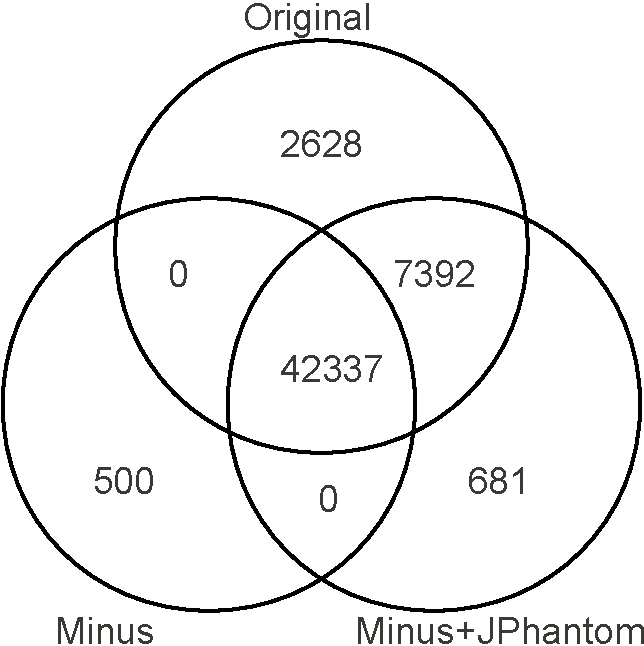
\includegraphics[scale=0.65]{figures/complementation/venn-crop.pdf}
  \caption[Reachable Methods Venn Diagram]{ A Venn diagram that shows
    how three different sets of reachable methods relate to each
    other. These three sets---(i) \emph{Original}, (ii) \emph{Minus},
    and (iii) \emph{Minus+JPhantom}---correspond to the outcomes of
    analyzing (i) the \emph{antlr} jar (original), (ii) the
    \emph{antlr-minus} jar (subset of the original jar), and (iii) the
    \emph{antlr-minus} jar after being transformed by JPhantom,
    respectively. The sets are not drawn to scale: the size of each
    subset is indicated only by the number in it.}
  \label{fig:venn}
\end{figure}

In summary, JPhantom avoids problems with crashes when encountering
phantom references as well as incompleteness when phantom references
are merely ignored. In practice, it is effective in discovering large
parts of the interface for missing methods and the produced complement
respects the requirements of the Java VM verifier, i.e., the most
fundamental Java well-formedness rules for types.


\subsection{Performance Experiments}

We use a 64-bit machine with a quad-core Intel i7 2.8GHz CPU. The
machine has 8GB of RAM. We ran our experiments using JDK 1.7
(64-bit).

Our benchmarks consist of%
\begin{inparaenum}[(1)]
\item \emph{antlr}, a parser generator,
\item \emph{antlrworks}, the GUI Development Environment for antlr,
\item \emph{c3p0}, a library that provides extensions to traditional
  JDBC drivers,
\item \emph{jruby} and
\item \emph{jython}, implementations of Ruby and Python programming
  languages respectively that run on top of the JVM,
\item logback-classic and
\item logback-core, two modules of the \emph{logback} logging
  framework,
\item \emph{pmd}, a Java source code analyzer,
\item \emph{postgres}, the PosgreSQL JDBC driver,
\item \emph{sablecc}, a compiler generator, and
\item \emph{antlr-minus}, a synthetic benchmark described in the
  previous section.
\end{inparaenum}
% in order to increase the number of constraints it produces.
Every benchmark is just a jar file that serves as JPhantom's
input, which then detects all phantom references and generates the
complemented jar.

We encountered most of these benchmarks in our own work doing static
program analysis with the Doop
framework \cite{BS-OOPSLA09,hybrid-pldi13}. For many of the benchmarks
it was, upon original encounter, an unexpected discovery that they
could not be analyzed due to dependencies to unknown classes in other
libraries.

Figure~\ref{fig:exp1} presents input features and the running time of
JPhantom for each of our benchmarks. The first column is the name of
the benchmark. The second column is the size of the output, i.e., the
complemented jar, divided into the original size of the input
(benchmark) and the size of the complement itself (i.e., the size of
the generated phantom classes). The third and fourth columns are the
number of phantom classes and constraints detected respectively. The
last column is the running time of JPhantom, including the time to
analyze the input, compute a type hierarchy that respects all of the
constraints detected, create the phantom classes with the required
members and supertypes, augment the input jar and flush its contents
to disk.

\begin{figure}[htp]
\centering
\small
\begin{savenotes}
\begin{tabular}{@{}l@{\hspace{1em}}r@{\ +\ }r@{\hspace{1em}}r@{\hspace{1em}}r@{\hspace{1em}}r@{}}
  \toprule
  %% \emph{Input jar} & \emph{Size} & \emph{Complement} &
  \emph{Input jar} & \multicolumn{2}{c}{\emph{Size}}  &
  \emph{Phantom} & \emph{Constraints} & \emph{Time} \\
  \midrule
  antlr & $3.3$M & $0.7$K & $1$ & $2$ & $4.82s$ \\ %% antlr-master-3.4.1-SNAPSHOT-completejar.jar (used to be 3.93)**
  antlrworks & $3.5$M & $2.2$K & $5$ & $7$ & $6.11s$ \\ %% antlrworks-1.5rc1.jar (used to be 5.12)
  c3p0 & $597$K & $1.8$K & $4$ & $2$ & $2.05s$ \\ %% c3p0-0.9.1.2.jar (used to be 1.86)
  jruby & $19$M & $5.9$K & $16$ & $20$ & $13.70s$ \\ %% jruby-complete-1.7.2.jar (used to be 12.06)
  jython & $2.5$M & $4.0$K & $8$ & $9$ & $3.26s$ \\ %% jython.jar (used to be 2.99)
  logback-classic & $247$K & $55$K & $148$ & $212$ & $1.76s$ \\ %% logback-classic.jar (used to be 1.55)
  logback-core & $358$K & $7.9$K & $22$ & $22$ & $1.61s$ \\ %% logback-core-1.0.9.jar (used to be 1.22)
  pmd & $1.2$M & $11$K & $28$ & $36$ & $2.62s$ \\ %% pmd.jar (used to be 2.25)
  postgres & $499$K & $0$ & $0$ & $0$ & $1.95s$ \\ %% postgresql-8.4-701.jdbc4.jar (used to be 1.56)
  sablecc & $306$K & $2.3$K & $5$ & $8$ & $1.59s$ \\ %% sablecc-3.2.jar (used to be 1.32)
  \midrule
  antlr-minus & $3.2$M & $17$K & $37$ & $103$ & $5.82s$ \\ %% antlr-final.jar (used to be 4.72)
  \bottomrule
\end{tabular}
\end{savenotes}
\caption{%
    Results of experiments.
}
\label{fig:exp1}
\end{figure}


%% The execution times presented above changed since we added an extra
%% pass to jphantom, to account for missing members of available
%% classes. That is, an available class may call a method or reference
%% a field declared in one of its supertypes. It may be the case that
%% the member was declared in a phantom supertype, and thus no
%% declaration for it exists in the available classes,
%% whatsoever. What we did is, try to perform a member lookup for any
%% reference of a type that has at least one phantom supertype. If the
%% lookup fails, we pick a phantom supertype and add a constraint
%% which states that this phantom supertype must declare the missing
%% member. To perform the lookup, we had to implement an extra pass
%% that stores all declared methods and fields of the available
%% classes.

Even the largest benchmark (jruby) takes seconds to
complete. Moreover, the size of the input is highly correlated with
the running time of JPhantom and much less correlated with the number
of constraints. This suggests that most of the time is spent on
reading and analyzing the input, rather than on the type hierarchy
solver. The only slight exception is the logback-classic benchmark,
which requires about 1.8 seconds to complete despite its small
size. This is due to the large number of phantom classes and
constraints this benchmark produces, which is to be expected since it
is built on top of logback-core (which is not supplied as part of the
input). This practice of creating such a strong dependency is probably
justified by logback's design. The framework implements the SLF4J
(Simple Logging Facade for Java) protocol, which acts as a common
interface for a variety of logging frameworks, and hides the actual
framework (called
\emph{binding}) to be used underneath. From both logback-classic and
antlr-minus we can see that JPhantom scales well as the number of
constraints increases.

To see the constraints and their solution for a benchmark instance,
consider the list below, which is the actual execution output of a
JPhantom run on the jruby benchmark:

\begin{alltt}\footnotesize
Phantom Classes Detected: \hfill{[constraint]}

org.apache.tools.ant.BuildException \hfill{must be a class}
org.apache.tools.ant.Task \hfill{must be a class}
org.apache.tools.ant.Project
org.apache.bsf.util.BSFFunctions \hfill{must be a class}
org.apache.bsf.util.BSFEngineImpl \hfill{must be a class}
org.apache.bsf.BSFException \hfill{must be a class}
org.apache.bsf.BSFManager \hfill{must be a class}
org.apache.bsf.BSFDeclaredBean \hfill{must be a class}
org.apache.bsf.BSFEngine
org.osgi.framework.Bundle \hfill{must be an interface}
org.osgi.framework.BundleReference
org.osgi.framework.FrameworkUtil \hfill{must be a class}
org.osgi.framework.BundleException
org.osgi.framework.BundleContext \hfill{must be an interface}
java.dyn.Coroutine \hfill{must be a class}
java.dyn.CoroutineBase

Constraints:

org.apache.bsf.BSFException <: Throwable
org.apache.tools.ant.BuildException <: Throwable
org.osgi.framework.BundleException <: Throwable
org.jruby.embed.bsf.JRubyEngine <:
  org.apache.bsf.util.BSFEngineImpl
org.jruby.embed.bsf.JRubyEngine <:
  org.apache.bsf.BSFEngine
org.jruby.ant.RakeTaskBase <: org.apache.tools.ant.Task
org.jruby.javasupport.bsf.JRubyEngine <:
  org.apache.bsf.BSFEngine
org.jruby.ext.fiber.CoroutineFiber$1 <:
  java.dyn.Coroutine
org.jruby.javasupport.bsf.JRubyEngine <:
  org.apache.bsf.util.BSFEngineImpl

Class Hierarchy
* class java.lang.Object
  * class org.apache.bsf.BSFManager
  * class org.osgi.framework.FrameworkUtil
  * class Throwable (implements java.io.Serializable)
    * class org.osgi.framework.BundleException
    * class org.apache.tools.ant.BuildException
    * class org.apache.bsf.BSFException
  * class org.apache.bsf.BSFDeclaredBean
  * class org.apache.bsf.util.BSFFunctions
  * class org.apache.tools.ant.Task
    * class org.jruby.ant.RakeTaskBase
  * class java.dyn.Coroutine
    * class org.jruby.ext.fiber.CoroutineFiber$1
  * class org.apache.bsf.util.BSFEngineImpl (implements
     org.apache.bsf.BSFEngine)
    * class org.jruby.javasupport.bsf.JRubyEngine
    * class org.jruby.embed.bsf.JRubyEngine

Interface Hierarchy
* interface org.osgi.framework.Bundle
* interface org.apache.bsf.BSFEngine
* interface java.io.Serializable
* interface org.osgi.framework.BundleContext
\end{alltt}

It is evident that the final hierarchy respects all of the reported
constraints. Some interesting points are that:%
\begin{inparaenum}[(i)]
\item \code{org.apache.bsf.BSFEngine} defaults to interface since no
  constraint determines whether it is actually an interface or a
  class,
\item \code{org.osgi.framework.BundleException} is inferred to be a
  class since it is a subtype of the class \code{Throwable}, and
\item two known classes, \code{org.jruby.javasupport.bsf.JRubyEngine}
  and \code{org.jruby.embed.bsf.JRubyEngine}, used as subtypes of
  interface \code{org.apache.bsf.BSFEngine}, add the latter to the
  supertypes of their phantom projection,
  \code{org.apache.bsf.util.BSFEngineImpl}.
\end{inparaenum}


%%% Local Variables:
%%% mode: latex
%%% TeX-master: "../thesis"
%%% End:
